
%% bare_jrnl.tex
%% V1.4b
%% 2015/08/26
%% by Michael Shell
%% see http://www.michaelshell.org/
%% for current contact information.
%%
%% This is a skeleton file demonstrating the use of IEEEtran.cls
%% (requires IEEEtran.cls version 1.8b or later) with an IEEE
%% journal paper.
%%
%% Support sites:
%% http://www.michaelshell.org/tex/ieeetran/
%% http://www.ctan.org/pkg/ieeetran
%% and
%% http://www.ieee.org/

%%*************************************************************************
%% Legal Notice:
%% This code is offered as-is without any warranty either expressed or
%% implied; without even the implied warranty of MERCHANTABILITY or
%% FITNESS FOR A PARTICULAR PURPOSE! 
%% User assumes all risk.
%% In no event shall the IEEE or any contributor to this code be liable for
%% any damages or losses, including, but not limited to, incidental,
%% consequential, or any other damages, resulting from the use or misuse
%% of any information contained here.
%%
%% All comments are the opinions of their respective authors and are not
%% necessarily endorsed by the IEEE.
%%
%% This work is distributed under the LaTeX Project Public License (LPPL)
%% ( http://www.latex-project.org/ ) version 1.3, and may be freely used,
%% distributed and modified. A copy of the LPPL, version 1.3, is included
%% in the base LaTeX documentation of all distributions of LaTeX released
%% 2003/12/01 or later.
%% Retain all contribution notices and credits.
%% ** Modified files should be clearly indicated as such, including  **
%% ** renaming them and changing author support contact information. **
%%*************************************************************************


% *** Authors should verify (and, if needed, correct) their LaTeX system  ***
% *** with the testflow diagnostic prior to trusting their LaTeX platform ***
% *** with production work. The IEEE's font choices and paper sizes can   ***
% *** trigger bugs that do not appear when using other class files.       ***                          ***
% The testflow support page is at:
% http://www.michaelshell.org/tex/testflow/



\documentclass[journal]{IEEEtran}
%
%\smartqed  % flush right qed marks, e.g. at end of proof
%
\usepackage{graphicx}
\usepackage{changes}
\usepackage{amssymb}
\usepackage{graphicx}
\usepackage{amsmath,amssymb,latexsym,float,epsfig,subfigure}
\usepackage{mathtools, bbm}
\usepackage{amsmath} % assumes amsmath package installed
\usepackage{amssymb}  % assumes amsmath package installed
\usepackage{lipsum}
\usepackage[export]{adjustbox}
\usepackage[normalem]{ulem} % underline
\usepackage{wrapfig}
\usepackage{multirow}
\usepackage{balance}
\usepackage{color}
\usepackage{url}
\usepackage{tablefootnote}
\usepackage{microtype}
\usepackage{algorithm, algorithmic}
\usepackage{breqn}
\usepackage[bottom]{footmisc}


\newcommand{\argmax}{\arg\!\max}
\newcommand{\norm}[1]{\left\lVert#1\right\rVert}
\newcommand{\DGc}[1]{{\textbf{\color{blue}{#1}}}}
\definechangesauthor{de}
%
% If IEEEtran.cls has not been installed into the LaTeX system files,
% manually specify the path to it like:
% \documentclass[journal]{../sty/IEEEtran}





% Some very useful LaTeX packages include:
% (uncomment the ones you want to load)


% *** MISC UTILITY PACKAGES ***
%
%\usepackage{ifpdf}
% Heiko Oberdiek's ifpdf.sty is very useful if you need conditional
% compilation based on whether the output is pdf or dvi.
% usage:
% \ifpdf
%   % pdf code
% \else
%   % dvi code
% \fi
% The latest version of ifpdf.sty can be obtained from:
% http://www.ctan.org/pkg/ifpdf
% Also, note that IEEEtran.cls V1.7 and later provides a builtin
% \ifCLASSINFOpdf conditional that works the same way.
% When switching from latex to pdflatex and vice-versa, the compiler may
% have to be run twice to clear warning/error messages.






% *** CITATION PACKAGES ***
%
%\usepackage{cite}
% cite.sty was written by Donald Arseneau
% V1.6 and later of IEEEtran pre-defines the format of the cite.sty package
% \cite{} output to follow that of the IEEE. Loading the cite package will
% result in citation numbers being automatically sorted and properly
% "compressed/ranged". e.g., [1], [9], [2], [7], [5], [6] without using
% cite.sty will become [1], [2], [5]--[7], [9] using cite.sty. cite.sty's
% \cite will automatically add leading space, if needed. Use cite.sty's
% noadjust option (cite.sty V3.8 and later) if you want to turn this off
% such as if a citation ever needs to be enclosed in parenthesis.
% cite.sty is already installed on most LaTeX systems. Be sure and use
% version 5.0 (2009-03-20) and later if using hyperref.sty.
% The latest version can be obtained at:
% http://www.ctan.org/pkg/cite
% The documentation is contained in the cite.sty file itself.






% *** GRAPHICS RELATED PACKAGES ***
%
\ifCLASSINFOpdf
  % \usepackage[pdftex]{graphicx}
  % declare the path(s) where your graphic files are
  % \graphicspath{{../pdf/}{../jpeg/}}
  % and their extensions so you won't have to specify these with
  % every instance of \includegraphics
  % \DeclareGraphicsExtensions{.pdf,.jpeg,.png}
\else
  % or other class option (dvipsone, dvipdf, if not using dvips). graphicx
  % will default to the driver specified in the system graphics.cfg if no
  % driver is specified.
  % \usepackage[dvips]{graphicx}
  % declare the path(s) where your graphic files are
  % \graphicspath{{../eps/}}
  % and their extensions so you won't have to specify these with
  % every instance of \includegraphics
  % \DeclareGraphicsExtensions{.eps}
\fi
% graphicx was written by David Carlisle and Sebastian Rahtz. It is
% required if you want graphics, photos, etc. graphicx.sty is already
% installed on most LaTeX systems. The latest version and documentation
% can be obtained at: 
% http://www.ctan.org/pkg/graphicx
% Another good source of documentation is "Using Imported Graphics in
% LaTeX2e" by Keith Reckdahl which can be found at:
% http://www.ctan.org/pkg/epslatex
%
% latex, and pdflatex in dvi mode, support graphics in encapsulated
% postscript (.eps) format. pdflatex in pdf mode supports graphics
% in .pdf, .jpeg, .png and .mps (metapost) formats. Users should ensure
% that all non-photo figures use a vector format (.eps, .pdf, .mps) and
% not a bitmapped formats (.jpeg, .png). The IEEE frowns on bitmapped formats
% which can result in "jaggedy"/blurry rendering of lines and letters as
% well as large increases in file sizes.
%
% You can find documentation about the pdfTeX application at:
% http://www.tug.org/applications/pdftex





% *** MATH PACKAGES ***
%
%\usepackage{amsmath}
% A popular package from the American Mathematical Society that provides
% many useful and powerful commands for dealing with mathematics.
%
% Note that the amsmath package sets \interdisplaylinepenalty to 10000
% thus preventing page breaks from occurring within multiline equations. Use:
%\interdisplaylinepenalty=2500
% after loading amsmath to restore such page breaks as IEEEtran.cls normally
% does. amsmath.sty is already installed on most LaTeX systems. The latest
% version and documentation can be obtained at:
% http://www.ctan.org/pkg/amsmath





% *** SPECIALIZED LIST PACKAGES ***
%
%\usepackage{algorithmic}
% algorithmic.sty was written by Peter Williams and Rogerio Brito.
% This package provides an algorithmic environment fo describing algorithms.
% You can use the algorithmic environment in-text or within a figure
% environment to provide for a floating algorithm. Do NOT use the algorithm
% floating environment provided by algorithm.sty (by the same authors) or
% algorithm2e.sty (by Christophe Fiorio) as the IEEE does not use dedicated
% algorithm float types and packages that provide these will not provide
% correct IEEE style captions. The latest version and documentation of
% algorithmic.sty can be obtained at:
% http://www.ctan.org/pkg/algorithms
% Also of interest may be the (relatively newer and more customizable)
% algorithmicx.sty package by Szasz Janos:
% http://www.ctan.org/pkg/algorithmicx




% *** ALIGNMENT PACKAGES ***
%
%\usepackage{array}
% Frank Mittelbach's and David Carlisle's array.sty patches and improves
% the standard LaTeX2e array and tabular environments to provide better
% appearance and additional user controls. As the default LaTeX2e table
% generation code is lacking to the point of almost being broken with
% respect to the quality of the end results, all users are strongly
% advised to use an enhanced (at the very least that provided by array.sty)
% set of table tools. array.sty is already installed on most systems. The
% latest version and documentation can be obtained at:
% http://www.ctan.org/pkg/array


% IEEEtran contains the IEEEeqnarray family of commands that can be used to
% generate multiline equations as well as matrices, tables, etc., of high
% quality.




% *** SUBFIGURE PACKAGES ***
%\ifCLASSOPTIONcompsoc
%  \usepackage[caption=false,font=normalsize,labelfont=sf,textfont=sf]{subfig}
%\else
%  \usepackage[caption=false,font=footnotesize]{subfig}
%\fi
% subfig.sty, written by Steven Douglas Cochran, is the modern replacement
% for subfigure.sty, the latter of which is no longer maintained and is
% incompatible with some LaTeX packages including fixltx2e. However,
% subfig.sty requires and automatically loads Axel Sommerfeldt's caption.sty
% which will override IEEEtran.cls' handling of captions and this will result
% in non-IEEE style figure/table captions. To prevent this problem, be sure
% and invoke subfig.sty's "caption=false" package option (available since
% subfig.sty version 1.3, 2005/06/28) as this is will preserve IEEEtran.cls
% handling of captions.
% Note that the Computer Society format requires a larger sans serif font
% than the serif footnote size font used in traditional IEEE formatting
% and thus the need to invoke different subfig.sty package options depending
% on whether compsoc mode has been enabled.
%
% The latest version and documentation of subfig.sty can be obtained at:
% http://www.ctan.org/pkg/subfig




% *** FLOAT PACKAGES ***
%
%\usepackage{fixltx2e}
% fixltx2e, the successor to the earlier fix2col.sty, was written by
% Frank Mittelbach and David Carlisle. This package corrects a few problems
% in the LaTeX2e kernel, the most notable of which is that in current
% LaTeX2e releases, the ordering of single and double column floats is not
% guaranteed to be preserved. Thus, an unpatched LaTeX2e can allow a
% single column figure to be placed prior to an earlier double column
% figure.
% Be aware that LaTeX2e kernels dated 2015 and later have fixltx2e.sty's
% corrections already built into the system in which case a warning will
% be issued if an attempt is made to load fixltx2e.sty as it is no longer
% needed.
% The latest version and documentation can be found at:
% http://www.ctan.org/pkg/fixltx2e


%\usepackage{stfloats}
% stfloats.sty was written by Sigitas Tolusis. This package gives LaTeX2e
% the ability to do double column floats at the bottom of the page as well
% as the top. (e.g., "\begin{figure*}[!b]" is not normally possible in
% LaTeX2e). It also provides a command:
%\fnbelowfloat
% to enable the placement of footnotes below bottom floats (the standard
% LaTeX2e kernel puts them above bottom floats). This is an invasive package
% which rewrites many portions of the LaTeX2e float routines. It may not work
% with other packages that modify the LaTeX2e float routines. The latest
% version and documentation can be obtained at:
% http://www.ctan.org/pkg/stfloats
% Do not use the stfloats baselinefloat ability as the IEEE does not allow
% \baselineskip to stretch. Authors submitting work to the IEEE should note
% that the IEEE rarely uses double column equations and that authors should try
% to avoid such use. Do not be tempted to use the cuted.sty or midfloat.sty
% packages (also by Sigitas Tolusis) as the IEEE does not format its papers in
% such ways.
% Do not attempt to use stfloats with fixltx2e as they are incompatible.
% Instead, use Morten Hogholm'a dblfloatfix which combines the features
% of both fixltx2e and stfloats:
%
% \usepackage{dblfloatfix}
% The latest version can be found at:
% http://www.ctan.org/pkg/dblfloatfix




%\ifCLASSOPTIONcaptionsoff
%  \usepackage[nomarkers]{endfloat}
% \let\MYoriglatexcaption\caption
% \renewcommand{\caption}[2][\relax]{\MYoriglatexcaption[#2]{#2}}
%\fi
% endfloat.sty was written by James Darrell McCauley, Jeff Goldberg and 
% Axel Sommerfeldt. This package may be useful when used in conjunction with 
% IEEEtran.cls'  captionsoff option. Some IEEE journals/societies require that
% submissions have lists of figures/tables at the end of the paper and that
% figures/tables without any captions are placed on a page by themselves at
% the end of the document. If needed, the draftcls IEEEtran class option or
% \CLASSINPUTbaselinestretch interface can be used to increase the line
% spacing as well. Be sure and use the nomarkers option of endfloat to
% prevent endfloat from "marking" where the figures would have been placed
% in the text. The two hack lines of code above are a slight modification of
% that suggested by in the endfloat docs (section 8.4.1) to ensure that
% the full captions always appear in the list of figures/tables - even if
% the user used the short optional argument of \caption[]{}.
% IEEE papers do not typically make use of \caption[]'s optional argument,
% so this should not be an issue. A similar trick can be used to disable
% captions of packages such as subfig.sty that lack options to turn off
% the subcaptions:
% For subfig.sty:
% \let\MYorigsubfloat\subfloat
% \renewcommand{\subfloat}[2][\relax]{\MYorigsubfloat[]{#2}}
% However, the above trick will not work if both optional arguments of
% the \subfloat command are used. Furthermore, there needs to be a
% description of each subfigure *somewhere* and endfloat does not add
% subfigure captions to its list of figures. Thus, the best approach is to
% avoid the use of subfigure captions (many IEEE journals avoid them anyway)
% and instead reference/explain all the subfigures within the main caption.
% The latest version of endfloat.sty and its documentation can obtained at:
% http://www.ctan.org/pkg/endfloat
%
% The IEEEtran \ifCLASSOPTIONcaptionsoff conditional can also be used
% later in the document, say, to conditionally put the References on a 
% page by themselves.




% *** PDF, URL AND HYPERLINK PACKAGES ***
%
%\usepackage{url}
% url.sty was written by Donald Arseneau. It provides better support for
% handling and breaking URLs. url.sty is already installed on most LaTeX
% systems. The latest version and documentation can be obtained at:
% http://www.ctan.org/pkg/url
% Basically, \url{my_url_here}.




% *** Do not adjust lengths that control margins, column widths, etc. ***
% *** Do not use packages that alter fonts (such as pslatex).         ***
% There should be no need to do such things with IEEEtran.cls V1.6 and later.
% (Unless specifically asked to do so by the journal or conference you plan
% to submit to, of course. )


% correct bad hyphenation here
\hyphenation{op-tical net-works semi-conduc-tor}


\begin{document}
%
% paper title
% Titles are generally capitalized except for words such as a, an, and, as,
% at, but, by, for, in, nor, of, on, or, the, to and up, which are usually
% not capitalized unless they are the first or last word of the title.
% Linebreaks \\ can be used within to get better formatting as desired.
% Do not put math or special symbols in the title.
\title{Active Intent Disambiguation for \\ Shared Autonomy Robots}
%
%
% author names and IEEE memberships
% note positions of commas and nonbreaking spaces ( ~ ) LaTeX will not break
% a structure at a ~ so this keeps an author's name from being broken across
% two lines.
% use \thanks{} to gain access to the first footnote area
% a separate \thanks must be used for each paragraph as LaTeX2e's \thanks
% was not built to handle multiple paragraphs
%
\author{Deepak~E.~Gopinath and Brenna~D.~Argall
%\author{Michael~Shell,~\IEEEmembership{Member,~IEEE,}
%        John~Doe,~\IEEEmembership{Fellow,~OSA,}
%        and~Jane~Doe,~\IEEEmembership{Life~Fellow,~IEEE}% <-this % stops a space
\thanks{Deepak E. Gopinath is with the Department of Mechanical Engineering, Northwestern University, Evanston, IL and the Shirley Ryan AbilityLab, Chicago, IL.} %
%\thanks{M. Shell was with the Department
%of Electrical and Computer Engineering, Georgia Institute of Technology, Atlanta,
%GA, 30332 USA e-mail: (see http://www.michaelshell.org/contact.html).}% <-this % stops a space
\thanks{Brenna D. Argall is with the Departments of Mechanical Engineering, Computer Science and Physical Medicine and Rehabilitation, Northwestern University, Evanston, IL., and the Shirley Ryan AbilityLab, Chicago, IL.}%
%\thanks{J. Doe and J. Doe are with Anonymous University.}% <-this % stops a space
\thanks{Manuscript received December 2, 2018. Revised on April 21, 2019.}}

% note the % following the last \IEEEmembership and also \thanks - 
% these prevent an unwanted space from occurring between the last author name
% and the end of the author line. i.e., if you had this:
% 
% \author{....lastname \thanks{...} \thanks{...} }
%                     ^------------^------------^----Do not want these spaces!
%
% a space would be appended to the last name and could cause every name on that
% line to be shifted left slightly. This is one of those "LaTeX things". For
% instance, "\textbf{A} \textbf{B}" will typeset as "A B" not "AB". To get
% "AB" then you have to do: "\textbf{A}\textbf{B}"
% \thanks is no different in this regard, so shield the last } of each \thanks
% that ends a line with a % and do not let a space in before the next \thanks.
% Spaces after \IEEEmembership other than the last one are OK (and needed) as
% you are supposed to have spaces between the names. For what it is worth,
% this is a minor point as most people would not even notice if the said evil
% space somehow managed to creep in.



% The paper headers
%\markboth{Journal of \LaTeX\ Class Files,~Vol.~14, No.~8, August~2015}%
\markboth{IEEE Transactions on Neural Systems and Rehabilitation Engineering, July 2019}
{\MakeLowercase{\textit{et al.}}: Bare Demo of IEEEtran.cls for IEEE Journals}
% The only time the second header will appear is for the odd numbered pages
% after the title page when using the twoside option.
% 
% *** Note that you probably will NOT want to include the author's ***
% *** name in the headers of peer review papers.                   ***
% You can use \ifCLASSOPTIONpeerreview for conditional compilation here if
% you desire.




% If you want to put a publisher's ID mark on the page you can do it like
% this:
%\IEEEpubid{0000--0000/00\$00.00~\copyright~2015 IEEE}
% Remember, if you use this you must call \IEEEpubidadjcol in the second
% column for its text to clear the IEEEpubid mark.



% use for special paper notices
%\IEEEspecialpapernotice{(Invited Paper)}




% make the title area
\maketitle

% As a general rule, do not put math, special symbols or citations
% in the abstract or keywords.
\begin{abstract}
Assistive shared-control robots have the potential to transform the lives of millions of people afflicted with severe motor impairments. The usefulness of shared-control robots typically relies on the underlying autonomy's ability to infer the user's needs and intentions, and the ability to do so \textit{unambiguously} is often a limiting factor for providing appropriate assistance confidently and accurately. The contributions of this paper are three-fold. First, we propose a \textit{goal disambiguation} algorithm that enhances the intent inference and assistive capabilities of a shared-control assistive robotic arm. Second, we introduce a field-theoretic approach to \textit{intent inference} inspired by dynamic field theory that works in tandem with the disambiguation scheme. Third, we present a pilot study with eight subjects to evaluate the efficacy of the disambiguation algorithm. Our results suggest that (a) the disambiguation system is of greater utility for more limited control interfaces and more complex tasks, and (b) subjects demonstrated a wide range of disambiguation request behaviors with the common thread of concentrating requests early in the execution.
%(c) there are no differences in the onset of the robot assistance between different mode switching paradigms across tasks or across interfaces. 
\end{abstract}

% Note that keywords are not normally used for peerreview papers.
\begin{IEEEkeywords}
Assistive Robotics, Shared Autonomy, Intent Inference, Intent Disambiguation
\end{IEEEkeywords}



% For peer review papers, you can put extra information on the cover
% page as needed:
% \ifCLASSOPTIONpeerreview
% \begin{center} \bfseries EDICS Category: 3-BBND \end{center}
% \fi
%
% For peerreview papers, this IEEEtran command inserts a page break and
% creates the second title. It will be ignored for other modes.
\IEEEpeerreviewmaketitle

\section{Introduction}
\IEEEPARstart{A}{ssistive} and rehabilitation machines---such as robotic arms and smart wheelchairs---have the potential to transform the lives of millions of people with severe motor impairments~\cite{laplante1992assistive}. With rapid technological advancements in the domain of robotics these machines have become more capable and complex, and with this complexity the control of these machines has become a greater challenge. 

The standard usage of these assistive machines relies on manual teleoperation typically enacted through a control interface such as a joystick. However, the greater the motor impairment of the user, the more limited are the interfaces available for them to use. These interfaces (for example, sip-and-puffs and switch-based head arrays) are low-dimensional and at times discrete and can typically only operate in subsets of the entire control space (referred to as \textit{control modes}). The dimensionality mismatch between the interface and the robot's controllable degrees-of-freedom (DoF) necessitates the user to switch between control modes during teleoperation and has been shown to add to the cognitive and physical burden and affects task performance negatively~\cite{herlant2016assistive}.
%\begin{figure}
%	\begin{center}
%		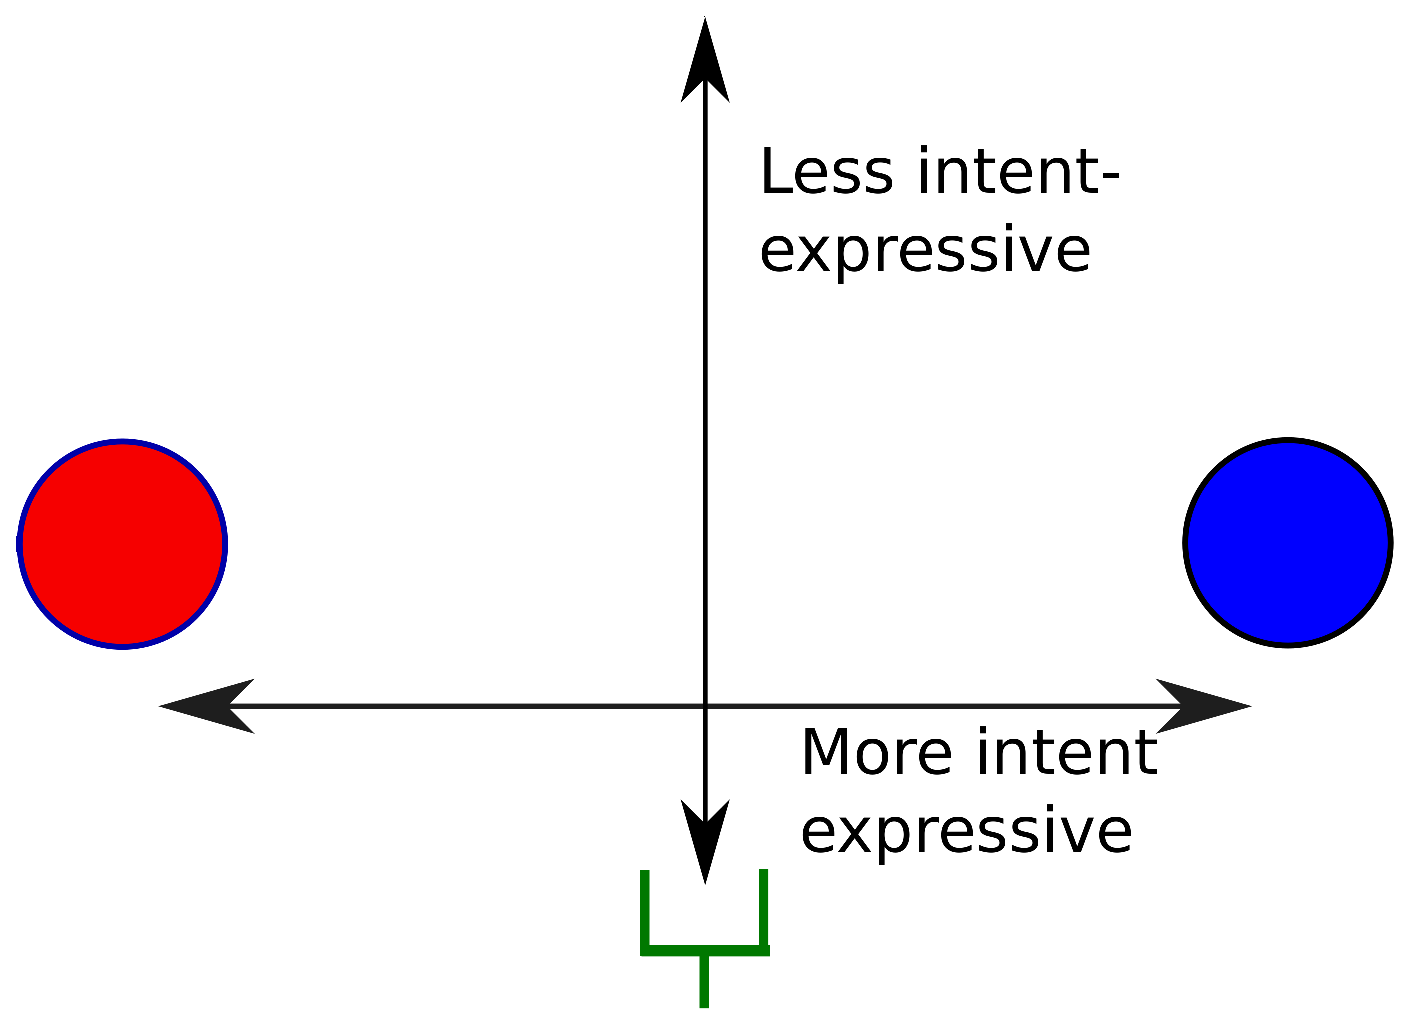
\includegraphics[width=0.35\textwidth]{./figures/Fig2.eps}
%	\end{center}
%	%	\vspace{-.45cm}
%	\caption{Illustration of goal disambiguation along various control dimensions. Any motion of the end effector (green) along the y-axis will not help the system to disambiguate the two goals (A and B). However, motion along the x-axis provides cues as to which goal.}
%	\label{fig:disamb}
%\end{figure}

The introduction of \textit{autonomy} to these assistive machines can alleviate some of the above-mentioned issues. More specifically, with \textit{shared} autonomy the task responsibility is shared between the user and the underlying autonomy. However, for autonomy to be effective in a shared setting, it needs to have a good idea of the user's needs and intentions. That is, \textit{intent inference} is critical to ensure appropriate assistance. 

In this work, we consider use-case scenarios in which the autonomy's inference of user intent is exclusively informed by the human's control commands issued via the control interface. As an example, in the domain of assistive robotic manipulation, these control commands are typically mapped to the end-effector (or joint) velocities and results in robot motion. Motion carries information regarding underlying intent. However, intent inference becomes particularly challenging when the user input is low-dimensional and sparse, as is the case with the more limited interfaces available to those with severe motor impairments. This is due to the fact that robot motion will likely be more discontinuous and jagged, and it might not carry information regarding underlying human intent. While to augment the human-robot system with high-fidelity sensors could be a straightforward approach to enhance the autonomy's intent inference capabilities in the assistive domain, user satisfaction and comfort is of paramount importance; furthermore additional sensors can quickly become cumbersome (e.g., if the sensors have to be worn by the user) and expensive. Therefore, for reasons of user adoption and cost, we intentionally design our assistance add-ons to be as invisible and close to the manual system as possible. The need for intent (goal) \textit{disambiguation} arises as the autonomy needs to reason about all possible goals before issuing appropriate assistance commands. 

%In assistive robotic manipulation specifically, often the first step of a manipulation task is to reach for and grasp discrete objects in the environment. Intent inference therefore can be framed as a problem of estimating a probability distribution of intent likelihood over all possible goals (objects) in the environment. Intent inference, typically, becomes more accurate with a greater number of sensor modalities available. However, due to reasons of user adoption and cost, for practical use-case scenarios we intentionally limit our assistance add-ons to be as invisible and close to the manual system as possible.

Our key insight in this work is that certain user control commands issued in certain control modes are \textit{more intent expressive} than others and therefore may help the autonomy to improve inference accuracy. 
%Consider the hypothetical reaching experiment illustrated in Figure~\ref{fig:disamb}. Since the spatial locations of the goals are maximally spread along the horizontal axis, any human control command issued along the horizontal dimension conveys a lot of information about the intended goal to the robot. In other words, motion along $x$ is more \textit{intent expressive} and will help the robot to draw accurate inference more quickly and confidently.
More specifically, in this work we investigate how the selection of a subset of the operational control dimensions or modes improves the intent inference and disambiguation capabilities of the robot. 
%As our primary contribution we develop a control mode selection algorithm which selects the control mode \textit{for} the user, in which the user-initiated motion will help the autonomy to \textit{maximally disambiguate} human intent by eliciting more \textit{intent expressive} control commands from the human. Furthermore, as the disambiguation power of our algorithm is closely linked to the fidelity of the underlying intent inference mechanism, as our secondary contribution we also propose a novel intent inference scheme based on ideas from \textit{dynamic field theory} in which the time-evolution of the distribution over goals is specified as continuous-time constrained dynamical system. 
The three main contributions of this work are as follows:
\begin{enumerate}
	\item First, we develop a control mode selection algorithm which selects the control mode \textit{for} the user, in which the user-initiated motion will help the autonomy to \textit{maximally disambiguate} human intent by eliciting more \textit{intent expressive} control commands from the human. In doing so, the autonomy will likely be able to assist the human more effectively and thereby improve overall task performance. This is important especially in the domain of assistive robotics wherein the user control commands are typically low-dimensional and sparse due to the inherent limitations of the control interfaces. 
	\item Second, as the disambiguation power of our algorithm is closely linked to the fidelity of the underlying intent inference mechanism, we also propose a field-theoretic approach to intent inference based on ideas from \textit{dynamic field theory} in which the time evolution of the probability distribution over goals is specified as a continuous-time constrained dynamical system \added{that obeys the \textit{principle of maximum entropy} in the absence of user control commands.}
	\item Third, we present results from a pilot study conducted to evaluate the efficacy of the disambiguation algorithm.
\end{enumerate}

In Section~\ref{sec:related-work} we present an overview of relevant research in the areas of shared autonomy in assistive robotics, intent inference, and synergies in human-robot interaction. Section~\ref{sec:ma} presents our mathematical formalism developed for intent disambiguation and inference. The study design and experimental methods are discussed in Section~\ref{sec:study_methods} followed by results in Section~\ref{sec:results}. Discussion and conclusions are presented in Sections~\ref{sec:discussion} and~\ref{sec:conclusions}.


\section{Related Work}\label{sec:related-work}
This section provides an overview of related research in the domains of shared autonomy in assistive robotics, intent inference in human-robot interaction, and synergies in human-robot interaction. 

Shared-autonomy in assistive systems aims to reduce the user's cognitive and physical burden during task execution, typically without having the user relinquish complete control~\cite{philips2007adaptive, demeester2008user, gopinath2017human, muelling2017autonomy}.
In order to offset the drop in task performance due to shifting focus (\text{task switching}) from the task at hand to switching between different control modes, various mode switch assistance paradigms have been proposed. For example, a simple time-optimal mode switching scheme has shown to improve task performance~\cite{herlant2016assistive, pilarski2012dynamic}. 

Shared control systems often require a good estimate of the human's intent---for example, their intended reaching target in a manipulation task or a target goal location in a navigation task~\cite{liu2016goal}. Intent can be explicitly communicated by the user~\cite{choi2008laser} via various modalities such as laser pointers, click interfaces and in some cases natural language. Intent can also be inferred from the user's control signals and other environmental cues using various algorithms. Within the context of shared autonomy a Bayesian scheme for user intent prediction models the user within the Markov Decision Process framework~\cite{dragan2012formalizing, javdani2017shared, admoni2016predicting} and is typically assumed to be noisily optimizing some cost function for their intended goal. In low-dimensional spaces, this cost function can be learned from expert demonstrations using Inverse Reinforcement Learning~\cite{ziebart2008maximum}. 

For high-dimensional spaces, such as that of robotic manipulation, learning cost functions that generalize well over the entire space requires large number of samples. In such cases, heuristic cost functions, such as sum of squared velocities along a trajectory, have been found to be useful for goal prediction~\cite{dragan2013policy}. Simple heuristic approaches can also be used to find direct mappings from instantaneous cues and the underlying human intention. Heuristic approaches can incorporate domain-specific knowledge easily and are computationally inexpensive, though the trade-off of this simplicity is not being sophisticated enough to incorporate histories of states and actions, making them less robust to external noise. Instantaneous confidence functions for estimating the intended reaching target are employed with success on multiple robotic manipulation systems~\cite{abbott2007haptic, gopinath2017human}. In our work we develop an inference algorithm that updates the belief over goals using ideas from dynamic field theory in which the histories of states and actions are incorporated using a single time-scale parameter and robustness to noise is ensured via recurrent self-interactions that stabilizes the dynamical system. 

From the robot's perspective, the core idea behind our intent disambiguation system is that of \textit{``Help Me, Help You''}---that is, if the user can help the robot with more intent-expressive actions, then the robot in turn can provide accurate and appropriate task assistance more accurately and confidently. More intent-expressive human actions also is related to the idea of legibility in robot actions. In human-robot interaction, the legibility and predictability of robot motion \textit{to} the human is investigated~\cite{dragan2013legibility} with various techniques to generate legible robot motion proposed ~\cite{holladay2014legible}. Our work relies on the idea of \textit{inverse legibility}~\cite{gopinath2017mode} in which the assistance scheme is intended to bring out more legible intent-expressive control commands \textit{from} the human. 


\section{Mathematical Formalism for Intent Disambiguation}\label{sec:ma}
This section describes our intent disambiguation algorithm, that computes the control mode that can maximally disambiguate between the goals, and our intent inference mechanism that works in conjunction with disambiguation algorithm. 

\subsection{Notation}
Let $\mathcal{G}$ denote the set of all candidate goals with $n_g = |\mathcal{G}|$ and let $g^i$ refer to the $i^{th}$ goal with $i \in [1,2,\dots,n_g]$. A \textit{goal} in this context represents the human's underlying intent. Specifically, in assistive robotic manipulation, since the robotic device first must reach toward and grasp discrete objects in the environment, intent inference is the estimation of the probability distribution over all possible discrete goals (objects) in the environment. At any time $t$, the autonomy maintains a probability distribution over goals denoted by $\boldsymbol{p}(t)$ such that $\boldsymbol{p}(t) = [p^1(t), p^2(t),\dots, p^{n_g}(t)]^{T}$ where $p^i(t)$ denotes the probability associated with goal $g^i$. The probability $p^i(t)$ represents the robot's confidence that goal $g^i$ is the human's intended goal.\footnote{By having the autonomy maintain a probability distribution over goals, we implicitly model the human as a Partially Observable Markov Decision Process (POMDP) in which all the uncertainty in the user's state is concentrated in the user's intended goal. By maintaining and updating a probability distribution over goals the autonomy can reason about the human's latent state (internal goal) during trial execution.  Inference over goal states is typically done using recursive Bayesian belief update which determines how the distribution evolves over time. In Section~\ref{sec:inference} we introduce a novel approach to compute the time evolution of probability distribution over goals that serves as an alternative to the recursive Bayesian update scheme.} 


Let $\mathcal{K}$ be the set of all controllable dimensions of the robot and $k^i$ represent the $i^{th}$ control dimension where $i \in [1,2,\dots,n_k]$ with $n_k = |\mathcal{K}|$. The limitations of the control interface necessitates $\mathcal{K}$ to be partitioned into control modes. Let $\mathcal{M}$ denote the set of all control modes with $n_m = \vert\mathcal{M}\vert$. Additionally, let $m^i$ refer to the $i^{th}$ control mode where $i \in [1,2,\dots,n_m]$. Each control mode $m^i$ is a subset of $\mathcal{K}$ such that $\bigcup\limits_{i=1}^{n_m} m^i$ spans all of the controllable dimensions. A dimension $k \in \mathcal{K}$ can be an element of multiple control modes.

%The cardinality of $\mathcal{K}$ is denoted as $n_k$ and typically depends on the robotic platform used. 
%For example, for a smart wheelchair $n_k = 2$, since the controllable degrees-of-freedom are velocity and heading. Likewise, for a six DoF robotic arm $n_k = 6$, since the controllable degrees-of-freedom correspond to the translation and rotation of the end-effector in the task-space. 

In this work, we assume a kinematic model for the robot and the kinematic state (the robot's end-effector pose) at any time $t$ is denoted as $\boldsymbol{x}_r(t) \in \mathbb{R}^3 \times \mathbb{S}^3$ and consists of a position and orientation component, where $\mathbb{S}^3$ is the space of all unit quaternions. The pose for goal $g \in \mathcal{G}$ is denoted as $\boldsymbol{x}_g \in \mathbb{R}^3 \times \mathbb{S}^3$. The control command issued by the human via the control interface is denoted as $\boldsymbol{u}_h$ and is mapped to the Cartesian velocity of the robot's end-effector. For a 6-DoF robotic arm, $\boldsymbol{u}_h \in \mathbb{R}^6$. The autonomous robot control policy that generates a robot control command is denoted as $\boldsymbol{u}_r \in \mathbb{R}^6$. The control command issued to the robot, which is a synthesis of $\boldsymbol{u}_h$ and $\boldsymbol{u}_r$ is denoted as $\boldsymbol{u} \in \mathbb{R}^6$. The control command that corresponds to a unit velocity vector along the positive and negative directions of control dimension $k$ is denoted as $\boldsymbol{e}^k$ and $-\boldsymbol{e}^k$ respectively.

\subsection{Disambiguation Metric}\label{ssec:disamb}
The disambiguation metric that we develop in this paper is a \textit{heuristic} measure that characterizes the intent disambiguation capabilities of a control dimension $k \in \mathcal{K}$ and is denoted as $D_k \in \mathbb{R}$. We explicitly define disambiguation metrics for both positive and negative motions along $k$ as $D_k^{+}$ and $D_k^{-}$ respectively. We also define a disambiguation metric $D_m \in \mathbb{R}$ for each control mode $m \in \mathcal{M}$.
By virtue of design, the disambiguation metric $D_m$ is a measure of how useful the user control commands would be \textit{for} the robot to perform more accurate intent inference if the user were to operate the robot in control mode $m$. Both $D_k$ and $D_m$ will be formally defined in Section~\ref{ssec:components}. 
Our computation of $D_k$ depends on four features (denoted as $\Gamma_k$, $\Omega_k$, $\Lambda_k$ and $\Upsilon_k$), that capture different aspects of the \textit{shape} of a projection of the probability distribution over intent. These projections and computations are described in detail in Section~\ref{ssec:projection} and Section~\ref{ssec:components}, and as pseudocode in Algorithm~\ref{alg1}. 

\subsection{Forward Projection of $\boldsymbol{p}(t)$}\label{ssec:projection}
The first step towards the computation of $D_k$ is model-based forward projection of the probability distribution $\boldsymbol{p}(t)$ from the current time $t_a$ to $t_b$ and $t_c$ (Algorithm~\ref{alg1}, lines 4-5) where $t_a < t_b < t_c$.\footnote{\textit{UpdateIntent()} in Line 4 is implemented using Equation~\ref{eq:dft_ii} discussed in detail in Section~\ref{ssec:dft_ii} and \textit{SimulateKinematics()} assumes a point-like robot kinematics.} We consider two future times in order to compute short-term ($t_b$) and long-term ($t_c$) evolutions of the probability distribution. Application of $\boldsymbol{e}^k$ results in probability distributions $\boldsymbol{p}^+_k(t_b)$, $\boldsymbol{p}^+_k(t_c)$ and $-\boldsymbol{e}^k$ results in $\boldsymbol{p}^-_k(t_b)$ and $\boldsymbol{p}^-_k(t_c)$, where the subscript $k$ captures the fact that the projection is the result of the application of a control command only along control dimension $k$. All parameters which affect the computation of $\boldsymbol{p}(t)$ are denoted as $\boldsymbol{\Theta}$. 
\begin{algorithm}[t]
	\caption{Intent Disambiguation}
	\label{alg1}
	\begin{algorithmic}[1]
		\REQUIRE $\boldsymbol{p}(t_a), \boldsymbol{x}_r(t_a), \Delta t, t_a < t_b < t_c, \boldsymbol{\Theta}$
		\FOR{$k=0\dots n_k$}
		\STATE Initialize $D_k = 0$, $t = t_a$, $\boldsymbol{u}_h = \boldsymbol{e}^k$
		
		\WHILE{$t \leq t_c$}
		\STATE $\boldsymbol{p}_k(t + \Delta t) \leftarrow \text{UpdateIntent}(\boldsymbol{p}_k(t), \boldsymbol{u}_h; \boldsymbol{\Theta})$
		\STATE $\boldsymbol{x}_r(t + \Delta t) \leftarrow \text{SimulateKinematics}(\boldsymbol{x}_r(t), \boldsymbol{u}_h)$
		\IF{$t = t_b$} \STATE {$Compute \;\;\Gamma_k, \Omega_k, \Lambda_k$} 
		\ENDIF
		\IF{$t = t_c$} \STATE{$Compute \;\;\Upsilon_k$} \ENDIF
		\STATE $t \leftarrow t + \Delta t$
		\ENDWHILE
		
		\STATE $Compute \;\;D_k$
		\ENDFOR
		
	\end{algorithmic}
\end{algorithm}

\subsection{Features of $D_k$}\label{ssec:components}
To compute our disambiguation metric, we design four features that encode different aspects of the \textit{shape} of the probability distribution as it evolves under user control in a specific control dimension $k$. For each control dimension $k$, each of the four features is computed for projections along both positive and negative directions independently. The four features are computed in lines 7 and 10 in Algorithm~\ref{alg1}.

1) \textit{Maximum:} The maximum of the projected probability distribution $\boldsymbol{p}_k(t_b)$ is a good measure of the robot's \textit{overall certainty} in accurately predicting human intent. We define the distribution maximum as
\begin{equation}
\Gamma_k = \max\limits_{1 \leq i \leq n_g}p^i_k(t_b)
\end{equation}
(i.e., the mode of this discrete distribution).
A higher value implies that the robot has a greater confidence in its prediction of the human's intended goal.

2) \textit{Pairwise separation:} More generally, disambiguation accuracy benefits from a larger separation, $\Lambda_k$, between goal probabilities. The quantity $\Lambda_k$ is computed as the \textit{sum of the pairwise distances} between the $n_g$ probabilities.
\begin{equation}
\Lambda_k = \sum_{i=1}^{n_g}\sum_{j=i}^{n_g}\lvert p^i_k(t_b) - p^j_k(t_b)\rvert
\end{equation}
$\Lambda_k$ is particularly helpful if the difference between the largest probabilities fails to disambiguate.

3) \textit{Difference between maxima:} Disambiguation accuracy benefits from greater differences between the first and second most probable goals. This difference is denoted as
\begin{equation}
\Omega_k = \text{max}(\boldsymbol{p}_k(t_b)) - \text{max}(\boldsymbol{p}_k(t_b) \setminus \text{max}(\boldsymbol{p}_k(t_b))) \;\;\;\;\;\;\;\;\;\;\;.
\end{equation}
$\Omega_k$ becomes particularly important when the distribution has multiple modes and a single measure of maximal certainty ($\Gamma_k$) alone is not sufficient for successful disambiguation. 

4) \textit{Gradients:} $\Gamma_k, \Omega_k$ and $\Lambda_k$ are local measures that encode shape characteristics of the short-term temporal projections of the probability distribution over goals. However, the quantity $\boldsymbol{p}_k(t)$ can undergo significant changes upon long-term continuation of motion along control dimension $k$. The spatial gradient of $\boldsymbol{p}_k(t)$ encodes this propensity for change and is approximated by 
\begin{equation*}
\frac{\partial\boldsymbol{p}_k(t)}{\partial x_k} \simeq \frac{\boldsymbol{p}_k(t_c) - \boldsymbol{p}_k(t_b)}{x_k(t_c) - x_k(t_b)}
\end{equation*}
where $x_k$ is the component of robot's projected displacement along control dimension $k$. The greater the difference between individual spatial gradients, the greater will the probabilities deviate from each other, thereby helping in disambiguation. In order to quantify the ``spread'' of gradients we define $\Upsilon_k$ as
\begin{equation}
\Upsilon_k = \sum_{i=1}^{n_g}\sum_{j=i}^{n_g}\Big \lvert\frac{\partial p^i_k(t)}{\partial x_k} - \frac{\partial p^j_k(t)}{\partial x_k}\Big \rvert
\end{equation}
where $\lvert\cdot\rvert$ denotes the absolute value. 

5) \textit{Putting it all together:} 
The individual features $\Gamma_k$, $\Omega_k$, $\Lambda_k$ and $\Upsilon_k$ are combined to compute $D_{k}$ in such a way that, by design, higher values of $D_k$ imply greater disambiguation capability for the control dimension $k$. More specifically, 
\begin{equation}\label{DK}
D_{k} = \underbrace{w\cdot(\Gamma_k\cdot \Lambda_k\cdot\Omega_k)}_{\text{short-term}} + \underbrace{(1 - w)\cdot \Upsilon_k}_{\text{long-term}}
\end{equation}
where $w$ is a task-specific weight that balances the contributions of the short-term and long-term components (in our implementation, $w$ is empirically set to $0.5$). Equation~\ref{DK} is computed twice, once in each of the positive ($\boldsymbol{e}^k$) and negative directions ($-\boldsymbol{e}^k$) along $k$, and the results ($D_k^+$ and $D_k^-$) are then summed to compute $D_k$. 

The computation of $D_k$ is performed for each control dimension $k \in \mathcal{K}$. The disambiguation metric $D_m$ for control mode $m$ then is calculated as 
\begin{equation*}\label{EQ2}
D_m = \sum_{k \in m} D_{k} \;
\end{equation*}
and the control mode with highest disambiguation capability $m^*$ is given by
\begin{equation*}
m^* = \argmax_m  D_{m}
\end{equation*}
while $k^* = \argmax_k D_k$ gives the control dimension with highest disambiguation capability $k^{*}$.
Disambiguation mode $m^{*}$ is the mode that the algorithm chooses \textit{for} the human to better estimate their intent. 
\section{Intent Inference}\label{sec:inference}

In this section, we propose a novel intent inference scheme inspired by \textit{dynamic field theory} in which the time evolution of the probability distribution $\boldsymbol{p}(t)$ is specified as a dynamical system with constraints. Section~\ref{ssec:dft} provides a primer on the basic principles and features of \textit{dynamic field theory} and its application in the fields of neuroscience and cognitive robotics. \added{Section~\ref{ssec:dft_ii} describes our formulation that makes use of dynamic field theory for the purposes of intent inference (Section~\ref{ssec:dft_adv}) presents the characteristics of the formulation and its applicability to assistive robotics and a simulation-based quantitative comparison of different goal inference methods. }
\subsection{Dynamic Field Theory}\label{ssec:dft}

In Dynamic Field Theory (DFT)~\cite{schoner2015dynamic}, variables of interest are treated as dynamical state variables. To represent the information about these variables requires two dimensions: one which specifies the value the variables can attain (the domain) and the other which encodes the \textit{activation level} or the amount of information about a particular value. These \textit{activation fields} (also known as dynamic neural fields) are analogous to probability distributions defined over a random variable. 

Following Amari's formulation~\cite{amari1977dynamics} dynamics of an activation field $\phi(x, t)$ are given by 
\begin{multline*}
\tau\frac{\partial{\phi}(x,t)}{\partial t} = -\phi(x,t) + h + S(x,t) + \\ \int\limits_{}^{}dx^{\prime}b(x-x^{\prime})\sigma(\phi(x^{\prime}, t)) 
\end{multline*} 
where $x$ denotes the variable of interest, $t$ is time, $\tau$ is the time-scale parameter, $h$ is the constant resting level, and $S(x,t)$ is the external input, $b(x-x^\prime)$ is the interaction kernel and $\sigma(\phi)$ is a sigmoidal nonlinear threshold function. The interaction kernel mediates how activations at all other field sites $x^\prime$ drive the activation level at $x$. Two types of interactions are possible: excitatory (when interaction is positive) which drives up the activation, and inhibitory (when the interaction is negative) which drives the activation down. 
Historically, dynamic neural fields originally were conceived to explain cortical population neuronal dynamics, based on the hypothesis that the excitatory and inhibitory neural interactions between local neuronal pools form the basis of cortical information processing. 
These activation fields possess some unique characteristics that make them ideal candidates for modeling higher-level cognition. First, a peak in the activation field can be \textit{sustained} even in the absence of external input due to the recurrent interaction terms. Second, information from the past can be \textit{preserved} over much larger time scales quite easily by tuning the time-scale parameter thereby endowing the fields with memory. Third, the activation fields are \textit{robust} to disturbance and noise in the external input~\cite{schoner2008dynamical}.
%As a result, DFT principles have found widespread application in the area of cognitive robotics~\citep{erlhagen2006dynamic}, specifically in the contexts of efficient human-robot interaction~\citep{erlhagen2014dynamic}, robotic scene representation~\citep{zibner2011dynamic}, obstacle avoidance and target reaching behaviors in both humans and robots~\citep{schoner1995dynamics}, and for object learning and recognition~\citep{faubel2008learning}. 

\subsection{Dynamic Neural Fields for Intent Inference}\label{ssec:dft_ii}
%The intent inference approach introduced in this section is inspired by \textit{Dynamic Field Theory} (DFT) in which the time evolution of the probability distribution $\boldsymbol{p}(t)$ is specified as a dynamical system with constraints. 

%Recurrent interaction between the state variables, robustness to noise, and inherent memory make dynamic neural fields an ideal candidate for an intent inference engine. 
Our insight is to use the framework of dynamic neural fields to specify the time evolution of the probability distribution $\boldsymbol{p}(t)$, in which we treat the individual goal probabilities $p^i(t)$ as constrained dynamical state variables such that $p^i(t) \in [0, 1]$ and $\Sigma_{1}^{n_g}p^{i}(t) = 1$. We refer to this approach as the \textit{field-theoretic intent inference.}
%The dynamical system can be generically written as 
%\begin{equation*}
%\frac{\partial \boldsymbol{p}(t)}{\partial t} = F(\boldsymbol{p}(t), \boldsymbol{u}_h ; \boldsymbol{\Theta})
%\end{equation*}
%where $F$ represents the nonlinear vector field, $\boldsymbol{u}_h$ is the human control input and $\boldsymbol{\Theta}$ represents all other task-relevant features and parameters that affect the time-evolution of the probability distribution. 
%Dynamic neural fields possess unique characteristics that make them ideal candidates for modeling higher-level cognition. 
%First, a peak in the activation field can be \textit{sustained} even in the absence of external input due to the recurrent interaction terms. Second, information from the past can be \textit{preserved} over large time scales quite easily by tuning the time-scale parameter, thereby endowing the variables with memory. Third, the activation fields are \textit{robust} to disturbance and noise in the external output~\cite{schoner2008dynamical}. 
%As a result, DFT principles have found widespread application in the area of cognitive robotics~\cite{erlhagen2006dynamic}, scene representation~\cite{zibner2011dynamic}, object learning and recognition~\cite{faubel2008learning}, and obstacle avoidance and target reaching behaviors in both humans and robots~\cite{schoner1995dynamics}. In the context of intent inference, the above-mentioned features result in smoother evolution of the belief over goals and avoid discontinuities in inference and can also incorporate information from distant past states quite easily. 

%\subsection{Dynamic Neural Fields for Intent Inference}\label{ssec:dnf_ii}

%We use the framework of dynamic neural fields to specify the time evolution of the probability distribution $\boldsymbol{p}(t)$, in which we treat the individual goal probabilities $p^i(t)$ as constrained dynamical state variables such that $p^i(t) \in [0, 1]$ and $\Sigma_{1}^{n_g}p^{i}(t) = 1$. 
%The dynamical system can be generically written as 
%\begin{equation*}
%\dot{\boldsymbol{p}}(t) = F(\boldsymbol{p}(t), \boldsymbol{u}_h ; \boldsymbol{\Theta})
%\end{equation*}
%where $F$ represents a nonlinear vector field, $\boldsymbol{u}_h$ is the human control input and $\boldsymbol{\Theta}$ represents all other task-relevant features that affect the time-evolution of the probability distribution. 
The full specification of the field is given by
%The time evolution of the probability distribution is given by
%\begin{multline}\label{eq:dft}
%\frac{\partial \boldsymbol{p}(t)}{\partial t} = \frac{1}{\tau}\bigg[-\mathbb{I}_{n_g\times n_g}\cdot\boldsymbol{p}(t) + \underbrace{\frac{1}{n_g}\cdot\mathbbm{1}_{n_g}\bigg]}_{\text{rest state}} \\+  \underbrace{\boldsymbol{\lambda}_{n_g\times n_g}\cdot\sigma(\boldsymbol{\xi}(\boldsymbol{u}_h;\boldsymbol{\Theta}))}_{\text{excitatory + inhibitory}}
%\end{multline}
%\begin{equation}
%\begin{equation*}
%\frac{\partial \boldsymbol{p}(t)}{\partial t} = \frac{1}{\tau}\bigg[-\mathbb{I}_{n_g\times n_g}\cdot\boldsymbol{p}(t) + \underbrace{\frac{1}{n_g}\cdot\mathbbm{1}_{n_g}\bigg]}_{\text{rest state}} 
%\end{equation*}
\begin{equation*}
\frac{\partial \boldsymbol{p}(t)}{\partial t} = \frac{1}{\tau_1}\bigg[\underbrace{-\boldsymbol{P}_{n_g\times n_g}\cdot\boldsymbol{p}(t)}_{\text{goal_transition_dynamics}}\bigg] +\frac{1}{\tau_2}\bigg[\underbrace{\frac{1}{n_g}\cdot\mathbbm{1}_{n_g}}_{\text{rest state}}\bigg]
\end{equation*}
%\begin{equation*}
%\frac{\partial \boldsymbol{p}(t)}{\partial t} = \frac{1}{\tau_1}\bigg[\underbrace{-\boldsymbol{P}_{n_g\times n_g}\cdot\boldsymbol{p}(t)}_{\text{goal transition dynamics}}\bigg] + \underbrace{\frac{1}{n_g\cdot\tau_2}\cdot\mathbbm{1}_{n_g}}}}_{\text{rest state}} 
%\end{equation*}
\begin{equation}\label{eq:dft_ii}
+  \underbrace{\boldsymbol{\lambda}_{n_g\times n_g}\cdot\sigma(\boldsymbol{\xi}(\boldsymbol{u}_h;\boldsymbol{\Theta}))}_{\text{excitatory + inhibitory}}
\end{equation}
%\end{equation}

where $\boldsymbol{u}_h$ is the human control input and $\boldsymbol{\Theta}$ represents all other task-relevant features, time-scale parameters $\tau_1, \tau_2$ determine the memory capacity and decay behavior, $\boldsymbol{P}_{n_g\times n_g}$ is the state transition matrix for the embedded Markov chain that models the goal transitions as jump processes, $\mathbbm{1}_{n_g}$ is a vector of dimension $n_g$ containing all ones, $\boldsymbol{\lambda}$ is the control matrix that controls the excitatory and inhibitory aspects, $\boldsymbol{\xi}$ is a function that encodes the nonlinearity through which human control commands and task features affect the time evolution, and $\sigma$ is a biased sigmoidal nonlinearity given by $\sigma(\boldsymbol{\xi}) = \frac{1}{1 + e^{-\boldsymbol{\xi}}} - 0.5$. 


Our design of $\boldsymbol{\xi}$ is informed by what features of the human control input and environment effectively capture the human's underlying intent. We choose the \textit{directedness} of the robot motion towards a goal, the \textit{agreement} between the human commands and robot autonomy, and the \textit{proximity} to a goal. The \textit{directedness} component looks at the shortest straight line path towards a goal $g$, whereas the \textit{agreement} serves as an indicator of how similar (measured as a dot product) the human and autonomy signals are to each other.
 One dimension $i$ of $\boldsymbol{\xi}$ is defined as 
\begin{multline*}
\xi^i(\boldsymbol{u}_h;\boldsymbol{x}_r, \boldsymbol{x}_{g^i}, \boldsymbol{u}_{r, g^i}) = \underbrace{\frac{1 + \eta}{2}}_{\text{directedness}} + \underbrace{\boldsymbol{u}_{h}^{rot}\cdot\boldsymbol{u}_{r,g^i}^{rot}}_{\text{agreement}}
\\+ \underbrace{\text{max}\Big(0, 1-\frac{\norm{\boldsymbol{x}_{g^i} - \boldsymbol{x}_r}}{R}\Big)}_{\text{proximity}}
\end{multline*}
where  $\eta = \frac{\boldsymbol{u}_h^{trans}\cdot(\boldsymbol{x}_{g^i} - \boldsymbol{x}_r)^{trans}}{\norm{\boldsymbol{u}_h^{trans}}\norm{(\boldsymbol{x}_{g^i} - \boldsymbol{x}_r)^{trans}}}$, $\boldsymbol{u}_{r,g^i}$ is the robot autonomy command for reaching goal $g^i$, $trans$ and $rot$ refer to the translational and rotational components of a command $\boldsymbol{u}$ or position $\boldsymbol{x}$,  $R$ is the radius of the sphere beyond which the proximity component is always zero, $\norm{\cdot}$ is the Euclidean norm and $\boldsymbol{\Theta} = \{\boldsymbol{x}_r, \boldsymbol{x}_{g^i}, \boldsymbol{u}_{r, g^i}\}$.
%Given the initial probability distribution at time $t_a$ Equation~\ref{eq:dft} can be solved numerically from $t \in [t_a, t_b]$ using a simple Euler algorithm with a fixed time-step $\Delta t$.
At every time-step, constraints on $p^i(t)$ are enforced such that $\boldsymbol{p}(t)$ is a valid probability distribution. 
The most confident goal $g^*$ is computed as $g^* = \argmax_i  p^i(t)$.

\subsection{\added{Field-Theoretic Intent Inference For Assistive Robotics}}\label{ssec:dft_adv}
\begin{figure}[b]
	\centering
	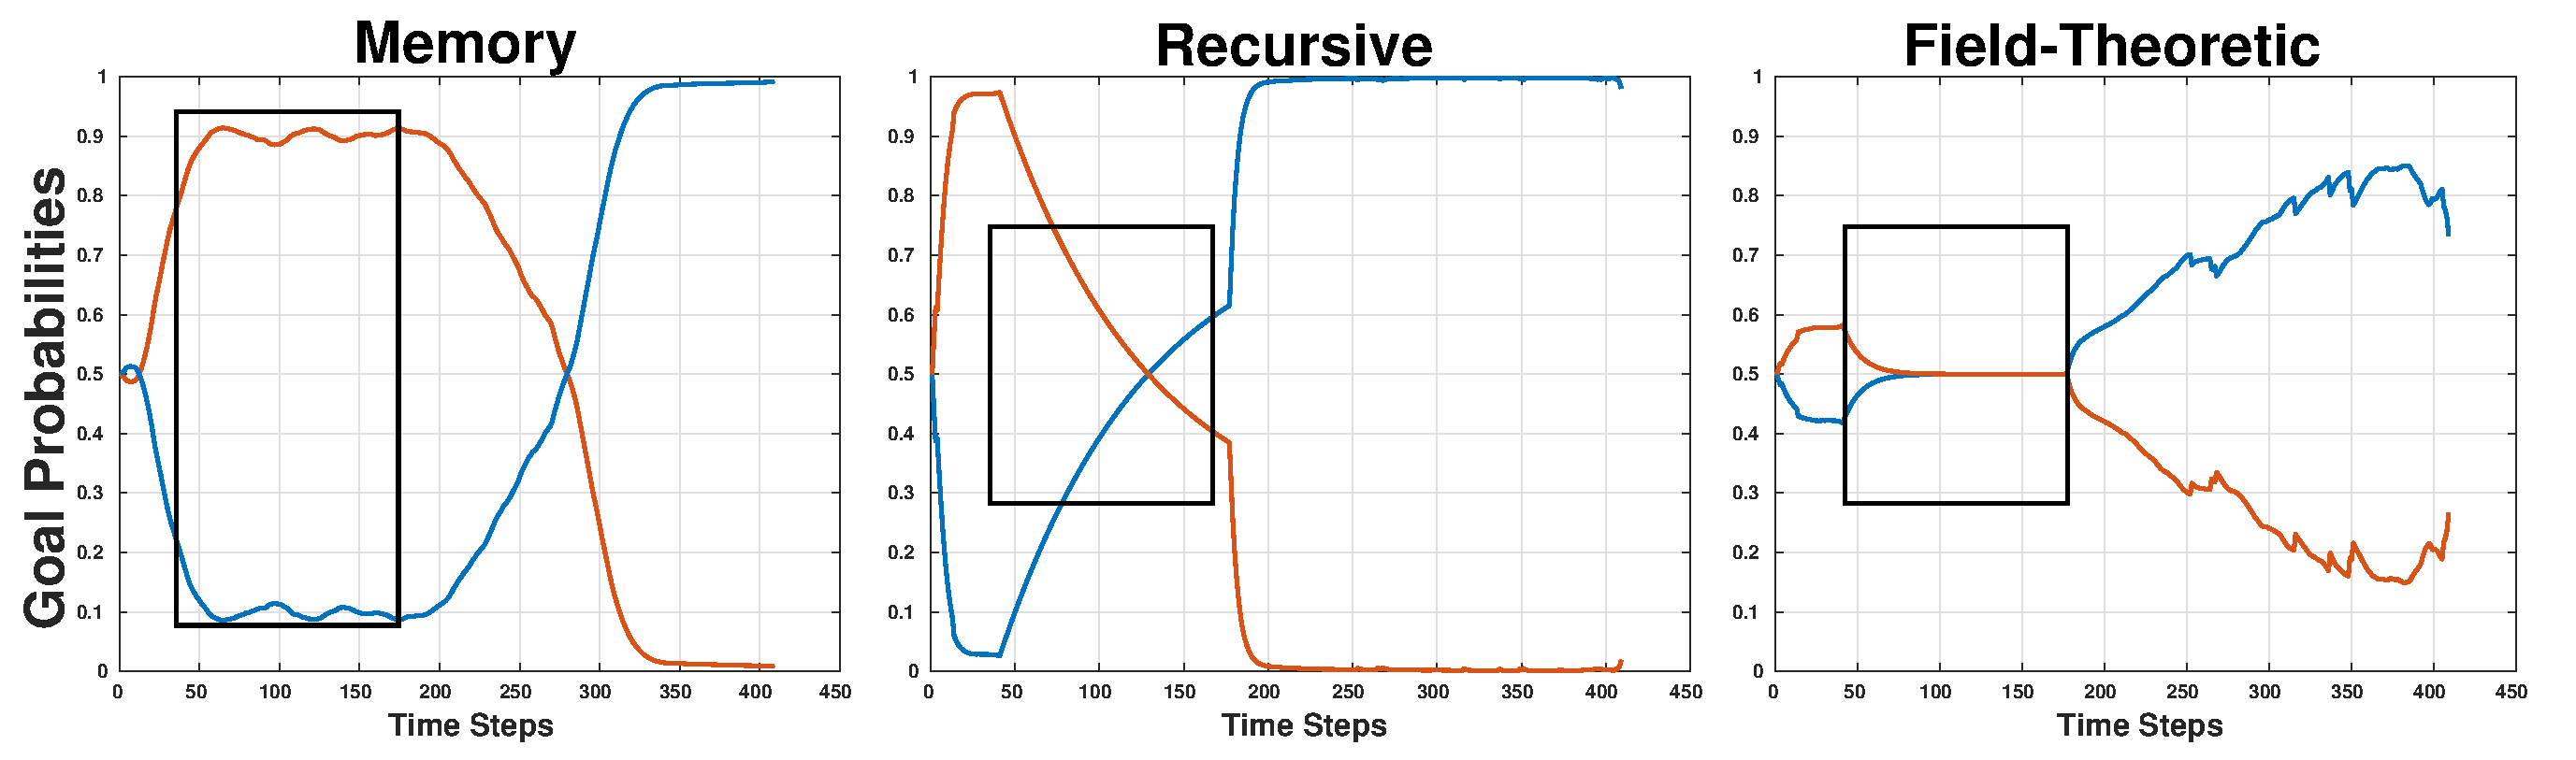
\includegraphics[width = 1.0\hsize]{./figures/inference_comparison_new.eps}
%	\vspace{-1cm}
	\caption{\added{Goal inference comparison: (Left to Right). Goal probabilities for Memory-Based Prediction (Left), Recursive Bayesian Belief Update (Middle) and DFT-based inference scheme (Right) and reaching behavior in a scene with two goals. The black boxes in the plots indicated time range during which the control velocity was zeroed. The probabilities do not change much for memory-based approach as the cost function employed is purely distance-based (left). The convergence is towards the stationary and uniform distribution for recursive (middle) and field-theoretic approach (right) respectively.}}
	\label{fig:dft_inference}
\end{figure}
\added{In our work, autonomy's inference of user intent solely relies on user control commands. In the domain of assistive robotics, it is quite often the case that the user input is highly discontinuous (due to fatigue, motor impairments, stoppage for mode switches \textit{et cetera}) due to which it becomes important to reason about belief over goals in the \textit{absence} of useful information. }

\added{In the absence of testable information (that is, no control commands issued by the user and not task-level global priors), in accordance to the \textit{maximum entropy principle}, the belief should converge to a uniform distribution. In the absence of $\boldsymbol{u}_h$ Equation~\ref{eq:dft_ii} converges to a uniform distribution mimicking natural forgetting behavior resulting in a more meaningful inference. The rate at which the distribution evolves to a uniform distribution is controlled by the timescale parameter $\tau_1$.}

\added{On the other hand, standard discrete-time recursive belief update equation as implemented in~\cite{jain2018recursive} is}
\begin{equation*}
p(g^t |\boldsymbol{u}_h^t) = \eta p(\boldsymbol{u}_h^t | g^t)\sum_{g^{t-1} \in \mathcal{G}}^{}p(g^t | g^{t-1})p(g^{t-1} |\boldsymbol{u}_h^{t-1})\;\;\;\;\;.
\end{equation*}
\added{where $\eta$ is the normalization factor, $\boldsymbol{p}(\boldsymbol{u}_h | g)$ is likelihood function, $p(g^t | g^{t-1})$ is the goal transition probability. 
In recursive belief update when $\boldsymbol{u}_h = 0$ with the likelihood function to be uniform, it can be shown that the posterior distribution over goals converges to the stationary distribution of the goal transition matrix. The stationary distribution is not necessarily uniform and therefore is counter-intuitive and can introduce unwanted biases in the inference. 
}

\added{
Knowledge of task-level semantics can provide informative global priors that can further improve the accuracy of the inference mechanism. Our field-theoretic approach can encode a task-level global prior in the `rest state' term. For example, in a multi-stage task such as pouring the contents of a cup into a bowl, the initial goal distribution will be biased towards the cup as it is more likely the target that the user would try to reach for. The relative values of $\tau_1$ and $\tau_2$ controls the convergence behavior (whether to uniform distribution or rest state distribution respectively) in the absence of $\boldsymbol{u}_h$.}

%
%On the contrary, DFT-based approach also offers the capability to encode task-level global priors in the `rest state' term. The relative values of $\tau_1$ and $\tau_2$ controls the convergence behavior (whether to uniform distribution or rest state distribution respectively) in the absence of $\boldsymbol{u}_h$.

\added{In order to evaluate the performance of the field-theoretic inference approach a point robot simulation-based quantitative comparison to 1) memory-based prediction~\cite{dragan2013policy} and 2) recursive belief updating~\cite{jain2018recursive} was implemented in $\mathbb{R}^3$. The human is modeled as issuing a control command that noisily optimizes a straight-line path towards the intended goal. Signal dropout was simulated by randomly zeroing out control commands. Additionally, $\boldsymbol{u}_h$ was set to be zero for a randomly chosen section of each trial in order to compare the convergence behavior of different approaches. The number of goals varied between three and five and goal transitions were randomly sampled every five to eight time steps. 500 trials were simulated. Inference accuracy is computed as the fraction of total trial time (excluding when $\boldsymbol{u}_h = 0$) for which an algorithm correctly inferred the ground truth. Results for DFT-based inference were comparable to recursive belief updating ($87.46\%$ and $87.43\%$ respectively) and outperformed memory-based prediction significantly ($59.15\%$). Figure~\ref{fig:dft_inference} shows an illustrative example of goal inference using the various methods. One can see that when there is no control command issued unlike the recursive belief approach, the field-theoretic approach converges to the maximum entropy uniform distribution.}



%Written in matrix form this becomes
%\begin{equation*}
%\boldsymbol{p}_t = \eta\boldsymbol{p}(\boldsymbol{u}_h | \boldsymbol{g}) \otimes \big[\boldsymbol{P}^{T}\cdot\boldsymbol{p}_{t-1}\big]
%\end{equation*}



%Figure~\ref{fig:dft_inference} shows an illustrative comparison of goal inferences using our DFT-based approach and two other Bayesian approaches i) memory-based prediction as implemented in~\cite{dragan2013policy} and ii) recursive belief updating as implemented in~\cite{jain2018recursive}.\footnote{For the memory-based inference scheme we use a straight-line distance based cost function and for the recursive belief update scheme we model the human as an approximately rational agent such that the $p(\boldsymbol{u}_h | g)$ is modeled as a von Mises distribution.}
%
%In the scenario shown in Figure~\ref{fig:dft_inference} (top row), the user teleoperates the end-effector in the three translational dimensions. The user initially moves the robot towards the black goal (on the left) and then changes direction to pursue the magenta goal (on the right). Subsequently, the user decides against going towards the magenta goal and decides to pursue the initial black goal by moving the end-effector to the left.
%
%In Figure~\ref{fig:dft_inference} we can see that (bottom row) the goal probabilities under our DFT-based inference mechanism evolve much more smoothly compared to the recursive belief update scheme thereby decreasing the possibility of false positives. Moreover, it is able to capture the change in user's intention back to the original goal and outperforms the memory-based prediction scheme. The choice of cost functions and likelihood functions have a significant impact on the performance of the memory-based and recursive belief update inference schemes. Overall the performance of DFT-based inference schemes are comparable to standard Bayesian approaches.


 
 
%Figure~\ref{fig:dft_inference} shows an illustrative comparison of goal inference using our DFT based approach and a Bayesian approach using a distance-based cost function used during shared autonomy operation. We found that, in general, both inference mechanisms consistently produced similar performances (intent prediction correctness) for a wide variety of goal configurations. In order to incorporate history of states, Bayesian approaches have to reason over the entire trajectory which can become computationally expensive, whereas in the DFT approach this is achieved by tuning the time-scale parameter. 

%For potential field $\gamma_g$, the attractor velocity is given by
%\begin{equation*}
%\dot{\boldsymbol{x}}_r^{attract} = \boldsymbol{x}_{g} - \boldsymbol{x}_r
%\end{equation*}
%where $\boldsymbol{x}_{g}$ is the location of goal $g$.\footnote{In position space, the `--' operator computes the difference between the goal position and current robot position in $\mathbb{R}^3$. In orientation space, the `--' operator computes the \textit{quaternion difference} between the goal orientation and the current robot orientation.} The repeller velocity is given by
%\begin{equation*}
%\dot{\boldsymbol{x}}_r^{repel} = \sum_{i \in \mathcal{G} \setminus g} \frac{\boldsymbol{x}_r - \boldsymbol{x}_{g^i}}{\mu(\norm{\boldsymbol{x}_r - \boldsymbol{x}_{g^i}}^2)}
%\end{equation*}
%where $\dot{\boldsymbol{x}}_r$ indicates the velocity of the robot in the world frame, $\mu$ controls the magnitude of the repeller velocity and $\norm{\cdot}$ is the Euclidean norm. 
%\begin{equation*}
%\boldsymbol{u}_{r,g} = \dot{\boldsymbol{x}}_r^{attract} + \dot{\boldsymbol{x}}_r^{repel} 
%\end{equation*}
%$\gamma_g$ 
%Furthermore, the position and orientation velocities are generated using independent potential fields. 

\section{Study Methods}\label{sec:study_methods}
In this section, we describe the study methods used to evaluate the efficacy of the disambiguation system. 

\noindent{\underline{\textbf{Participants:}}} For this study eight subjects were recruited (mean age: $31 \pm 11$, 3 males and 5 females). All participants gave their informed, signed consent to participate in the experiment, which was approved by Northwestern University's Institutional Review Board.

\noindent{\underline{\textbf{Hardware:}}} The experiments were performed using the MICO 6-DoF robotic arm (Kinova Robotics, Canada), specifically designed for assistive purposes. The software system was implemented using the Robot Operating System (ROS) and data analysis was performed in MATLAB. 
The subjects teleoperated the robot using two different control interfaces: a 2-axis joystick and a switch-based head array, controlling the 6D Cartesian velocities of the end-effector (Figure~\ref{fig:interfaces}). An external button was provided to request the mode switch assistance. 

In detail, the joystick generated 2D continuous control signals. Under joystick control the full control space was partitioned into five control modes that were accessed via button presses. 	
The switch-based head array consisted of three switches embedded in the headrest, operated via head movements and generated 1D discrete signals. Under head array control the full control space was partitioned into seven control modes, the back switch was used to cycle between the different control modes, and the switches to the left and right controlled the motion of the robot's end effector in the positive and negative directions along a selected control dimension.
\begin{figure}[b]
	\centering
	\includegraphics[width = 1\hsize]{./figures/Fig6_New.eps}
	%	\vspace{-0.35cm}
	\caption{A 2-axis joystick (left) and switch-based head array (center) and their operational paradigms (right). $v$ and $\omega$ indicate the translational and rotational velocities of the end-effector, respectively. }
	\label{fig:interfaces}
\end{figure}
\begin{figure}[ht!]
	\includegraphics[keepaspectratio, width = \textwidth/2 ]{./figures/Fig7.eps}
	\caption{Study tasks performed by subjects. \textit{Left:} Single-step reaching task. \textit{Right:} Multi-step pouring task. }
	\label{fig:tasks}
\end{figure}

\noindent{\underline{\textbf{Tasks:}}} Two different task types were evaluated.

\underline{\textit{Single-step:}} The aim was to reach one of five objects on the table, each with a target orientation (Figure~\ref{fig:tasks}, Left). 

\underline{\textit{Multi-step:}} Each trial began with a full cup held by the robot gripper. The task required first that the contents of the cup be poured into one of two containers, and then that the cup be placed at one of the two specified locations and with a specific orientation (Figure~\ref{fig:tasks}, Right). 

\noindent{\underline{\textbf{Switching Paradigms:}}} Two kinds of mode switching paradigms were evaluated in the study.

\underline{\textit{Manual}}: During task execution the user performed all mode switches. 

\underline{\textit{Disambiguation}}: The user either performed a mode switch manually or requested a switch to a \textit{disambiguation} mode. The user was free to issue disambiguation requests at any time during task execution, upon which the algorithm identified and switched the current control mode to the best disambiguating mode $m^*$ by invoking Algorithm~\ref{alg1}. It has to be noted that the user was also allowed to switch control modes using a manual mode switch any time as well. However, the user was required to request disambiguation at least once during the task execution. 


\noindent{\underline{\textbf{Shared Control:}}} Autonomy assistance was always active for both mode switch assistance (manual and disambiguation) paradigms. We used a blending-based shared-control paradigm in which the final robot control command was a linear composition of the human control command and an autonomous robot policy. With blending the amount of assistance was directly proportional to the probability of the most confident goal $g^*$, and thus to the strength of the intent inference. The probability distribution over goals, $\boldsymbol{p}(t)$, was updated using Equation~\ref{eq:dft_ii} outlined in Section~\ref{ssec:dft_ii} and the most confident goal was computed as $\argmax_i  p^i(t)$. Therefore, if intent inference improved as a result of goal disambiguation, more assistance would be provided by the robot.

Specifically, the autonomous control policy generates control command $\boldsymbol{u}_r \leftarrow f_{a}(\boldsymbol{x}_r)$
where $f_{a}(\cdot) \in \mathcal{F}_{a}$, and $\mathcal{F}_{a}$ was the set of all control behaviors corresponding to different tasks. This set could be derived using a variety of techniques such as \textit{Learning from Demonstrations}~\cite{argall2009survey, schaal1997learning}, motion planners~\cite{hsu2002randomized,ratliff2009chomp} or navigation functions~\cite{rimon1992exact,tanner2003nonholonomic}.
In our implementation, the autonomy's control command was generated using a simple potential field which is defined in all parts of the state space~\cite{khatib1986real}. Every goal $g$ was associated with a potential field $\gamma_g$ which treats $g$ as an attractor and all the other goals in the scene as repellers. The autonomy command was computed as a summation of the attractor and repeller velocities and operated in the full 6D Cartesian space. 

Let $\boldsymbol{u}_{r,g}$ be the autonomy command associated with goal $g$. Under blending, the final control command $\boldsymbol{u}$ issued to the robot then was given by
\begin{equation*}
\boldsymbol{u} = \alpha\cdot \boldsymbol{u}_{r,g^*} + (1 - \alpha)\cdot \boldsymbol{u}_h
\end{equation*}
where $g^*$ was the most confident goal. Similar to $\boldsymbol{u}_h$, the autonomy command $\boldsymbol{u}_{r, g^*} \in \mathbb{R}^6$ is mapped to the 6D Cartesian velocity of the end-effector. 
The blending factor $\alpha$ was a piecewise linear function of the probability $p(g^*)$ associated with $g^*$ and was given by
$$
\alpha = \left\{
\begin{array}{ll}
0 & \quad\quad~~~ p(g^*) \leq \rho_1 \\
\frac{\rho_3 (p(g^*) - \rho_1)}{\rho_2 - \rho_1}  &  \quad \text{if}\quad \rho_1 < p(g^*) \leq \rho_2  \\
\rho_3 & \quad\quad~~~ p(g^*) > \rho_2 	
\end{array}
\right.
$$
with $\rho_i \in [0, 1] \;\forall\; i \in [1,2,3]$ and $ \rho_2 > \rho_1$. 
In our implementation, we empirically set $\rho_1 = \frac{1.2}{n_g}, \rho_2 = \frac{1.4}{n_g}$ and $ \rho_3 = 0.7$.

\noindent{\underline{\textbf{Study protocol:}}} A within-subjects study was conducted using a fractional factorial design in which the manipulated variables were the tasks, control interfaces and the switching paradigm conditions. Each subject underwent an initial training period that lasted approximately 30 minutes. 

The training period consisted of three phases and two different task configurations. The subjects used both interfaces to perform the training tasks.

\underline{\textit{Phase One}}: The subjects were asked to perform a simple reaching motion towards a single goal in the scene. This phase was intended for the subjects to get familiarized with the control interface mappings and teleoperation of the robotic arm.

\underline{\textit{Phase Two}}: In the second phase of training, subjects experienced how the blending-based autonomy provided assistance during task execution. 
%The subjects were informed that blending assistance would be present for all trials of the experiment. 

\underline{\textit{Phase Three}}: For the third phase of the training, multiple objects were introduced in the scene. Subjects were able to explore the disambiguation request feature during a reaching task, to observe the effects of the mode switch request and subsequent change in robot assistance. 
Subjects were explicitly informed by the experimenter that upon a disambiguation request the robot will select a control mode that would help the autonomy figure out which goal the subject was going for and thereby enable it to assist the user more effectively.


During the testing phase, each subject performed both tasks using both interfaces under the \textit{Manual} and \textit{Disambiguation} paradigms. All trials started in a randomized initial control mode and robot position. The ordering of control interfaces and paradigms was randomized and counterbalanced across all subjects. Three trials were collected for the \textit{Manual} paradigm and five trials for the \textit{Disambiguation} paradigm. Each trial lasted approximately 10-40s depending on the starting position of the robot and the specified reaching target. At the start of each trial, $\boldsymbol{p}(t)$ was initialized as $\frac{1}{n_g}\cdot\mathbbm{1}_{n_g}$. During the trial as the user teleoperated the robot by generating control commands using the specified control interface, $\boldsymbol{p}(t)$ was updated according to Equation~\ref{eq:dft_ii} in an online fashion at each time step. Figure~\ref{fig:exp_block_diagram} captures how a single trial unfolds in time.

\begin{figure}[ht!]
	\centering
	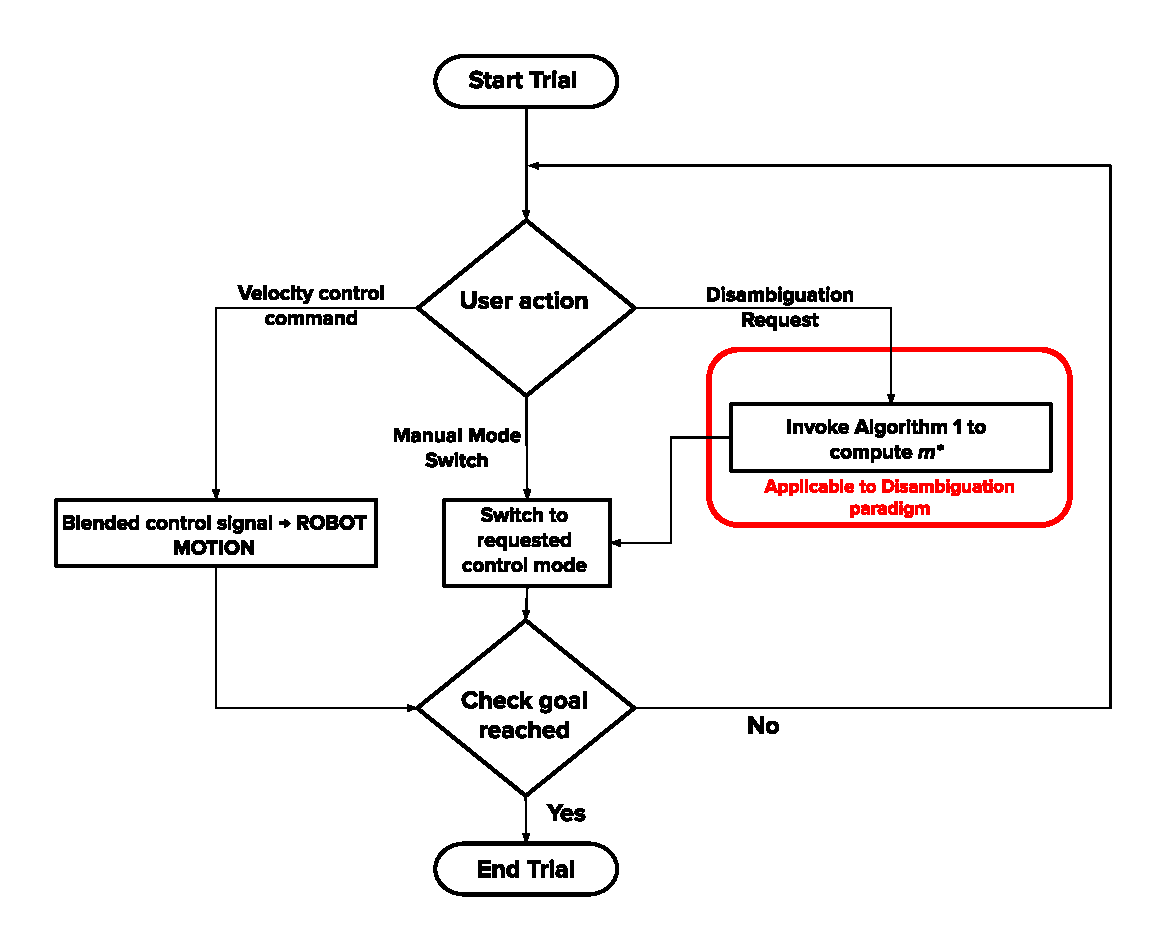
\includegraphics[keepaspectratio, width = 1.\hsize, height = 0.4\vsize, left]{./figures/ExperimentBlockDiagram.eps}
	\caption{Flow chart depicting user action sequence during a single trial. The user can issue three types of actions: a) Velocity control command b) Manual mode switch using a button press and c) Disambiguation request using a button press. Option a) results in online intent inference followed by generation of autonomy signal and blended control signal and subsequently causes robot motion. Options b) and c) lead to a control mode switch. At every timestep, the autonomy checks for the goal condition and decides whether to terminate the trial or not.}
	\label{fig:exp_block_diagram}
\end{figure}

\noindent{\underline{\textbf{Metrics:}}}
The objective metrics used for evaluation included the following. 
\begin{itemize}
	\item \textit{Number of mode switches}: The number of times a user switched between various control modes during task execution. This metric captures one of the main factors that contributes to the cognitive and physical effort required for task execution in assistive robotic manipulation~\cite{herlant2016assistive}.
	\item \textit{Number of disambiguation requests}: The number of times user pressed the disambiguation request button. 
	\item \textit{Number of button presses}: The sum of \textit{Number of mode switches} and \textit{Number of disambiguation requests}.
	\item \textit{Skewness}: A higher-order moment used to quantify the asymmetry of any distribution. Used to characterize how much the temporal distribution of disambiguation requests deviates from a uniform distribution. 
	\item \textit{\added{Task Completion Time}}: \added{Time taken to complete the task successfully and is an indicator of how well the human and autonomy work together.}
\end{itemize}

\added{Additionally, at the end of each testing phase, subjective data was gathered via a brief questionnaire. Users were given the following statements regarding the usefulness and capability of the assistance system to rate according to their agreement.
}
\begin{itemize}
	\item \textbf{Q1} - \added{Control modes chosen by the system made task execution easier.}
	\item \textbf{Q2} - \added{I liked operating the robots in the control modes chosen by the system.}
	\item \textbf{Q3} - \added{The robot and I worked together to accomplish the task.}
	\item \textbf{Q4} - \added{Which interface was the hardest to operate? 1-Joystick, 2-Head array.}
	\item \textbf{Q5} - \added{For which interface was the assistance paradigm the most useful 1-Joystick, 2-Head array.}
	\item \textbf{Q6} - \added{Which one of the schemes do you prefer the most? 1-Manual, 2-Disambiguation}
	\item \textbf{Q7} - \added{Which one of the schemes is the most user-friendly? 1-Manual, 2-Disambiguation}
\end{itemize}
\added{A 7-point Likert scale was used to rate \textbf{Q1-3} and for \textbf{Q4-Q7} subjects were required to pick one of the two given options. }

%\textit{Number of mode switches}: the number of times a user switched between various control modes during task execution. \textit{Number of disambiguation requests}: the number of times user pressed the disambiguation request button. \textit{Skewness}: a higher-order moment used to quantify the asymmetry of any distribution is used to characterize how much the temporal distribution of disambiguation requests deviates from a uniform distribution. Larger positive values of skewness correlate with more concentrated and earlier disambiguation requests. \textit{Number of button presses} is the sum of \textit{Number of mode switches} and \textit{Number of disambiguation requests}, and is also an indirect measure of user effort. 
%\textit{Onset of robot assistance} refers to the earliest time at which blending assistance to became active. 
%We also characterize the temporal distribution of disambiguation requests using a skewness measure. 
\section{Results}\label{sec:results}
\begin{figure}[b]
	\centering
	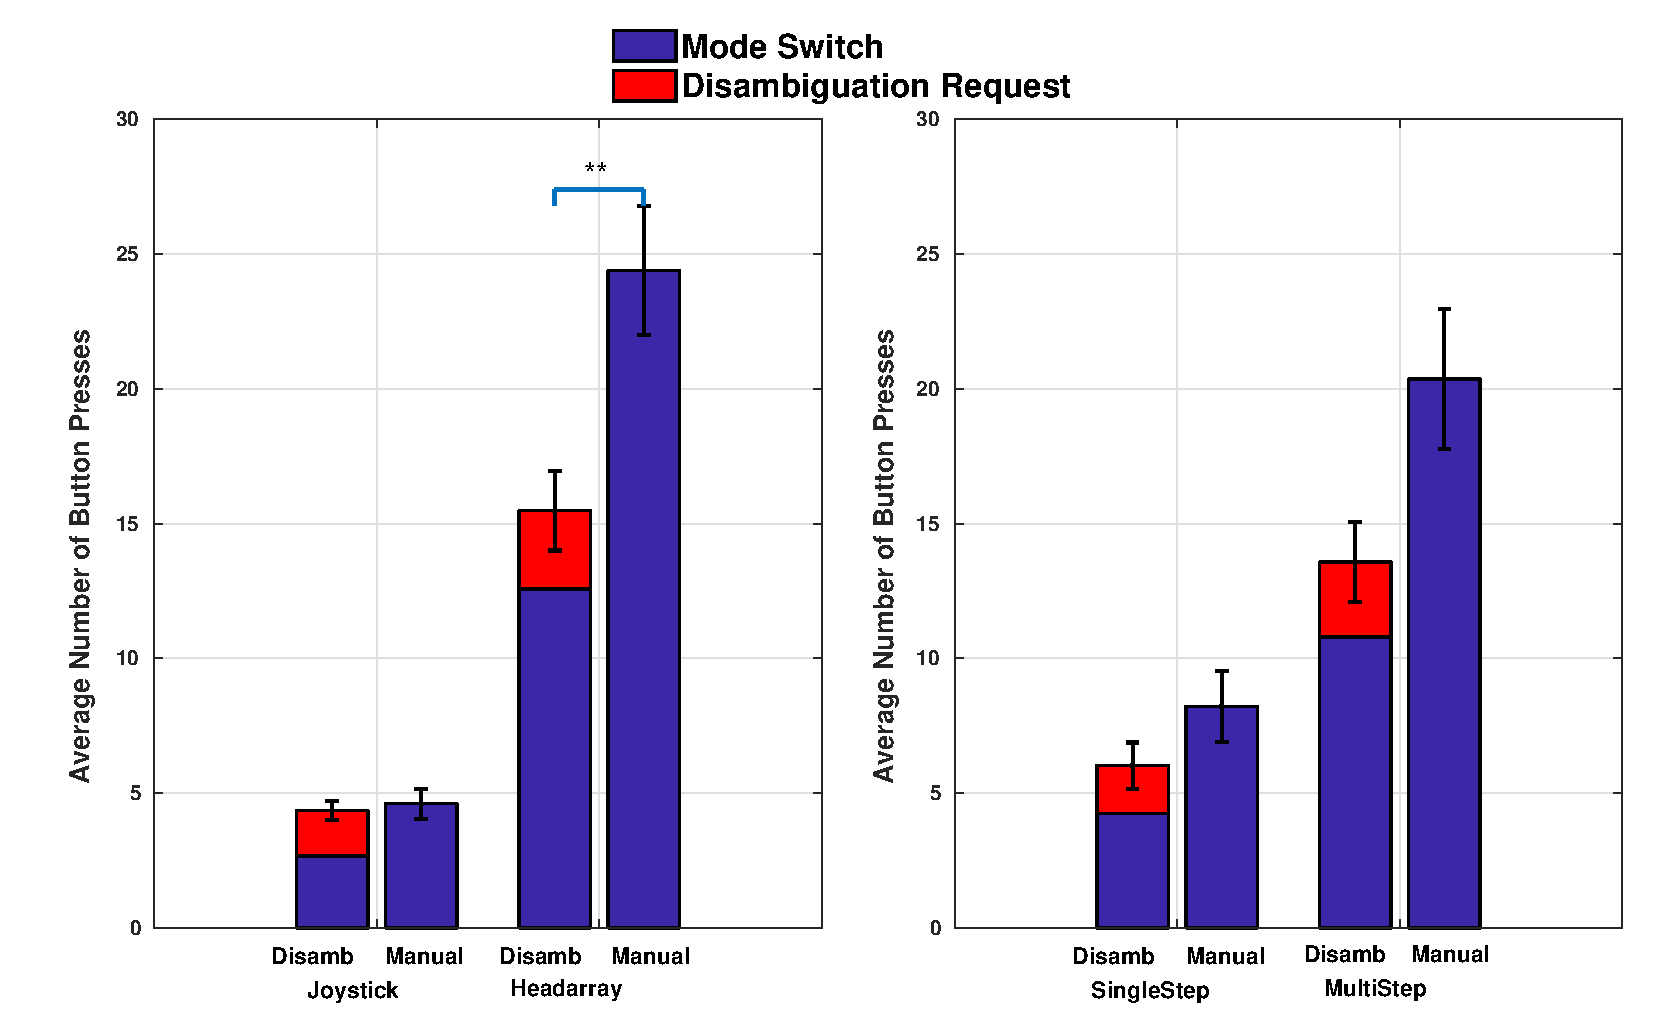
\includegraphics[keepaspectratio, width = 1\hsize ,left]{./figures/Fig8_New.eps}
	\caption{Comparison of average number of button presses between \textit{Disambiguation} and \textit{Manual} Paradigms. \textit{Left:} Grouped by control interfaces. \textit{Right:} Grouped by tasks.}
	\label{fig:button_press}
\end{figure}
Here we report the results of our subject study. Our study results indicated that the disambiguation request system is of greater utility for more limited control interfaces and more complex tasks and subjects demonstrated a wide range of disambiguations request behaviors with a common theme of relying on disambiguation assistance early in the trials. \added{Furthermore, the survey results showed that operating the robot in the disambiguating modes made task execution easier and that users preferred the \textit{Disambiguation} paradigm to the \textit{Manual} paradigm.} Statistical significance was determined by the Wilcoxon Rank-Sum test in where (***) indicates $p < 0.001$, (**) $p < 0.01$ and (*) $p < 0.05$.
\begin{figure}[t!]
	\centering
	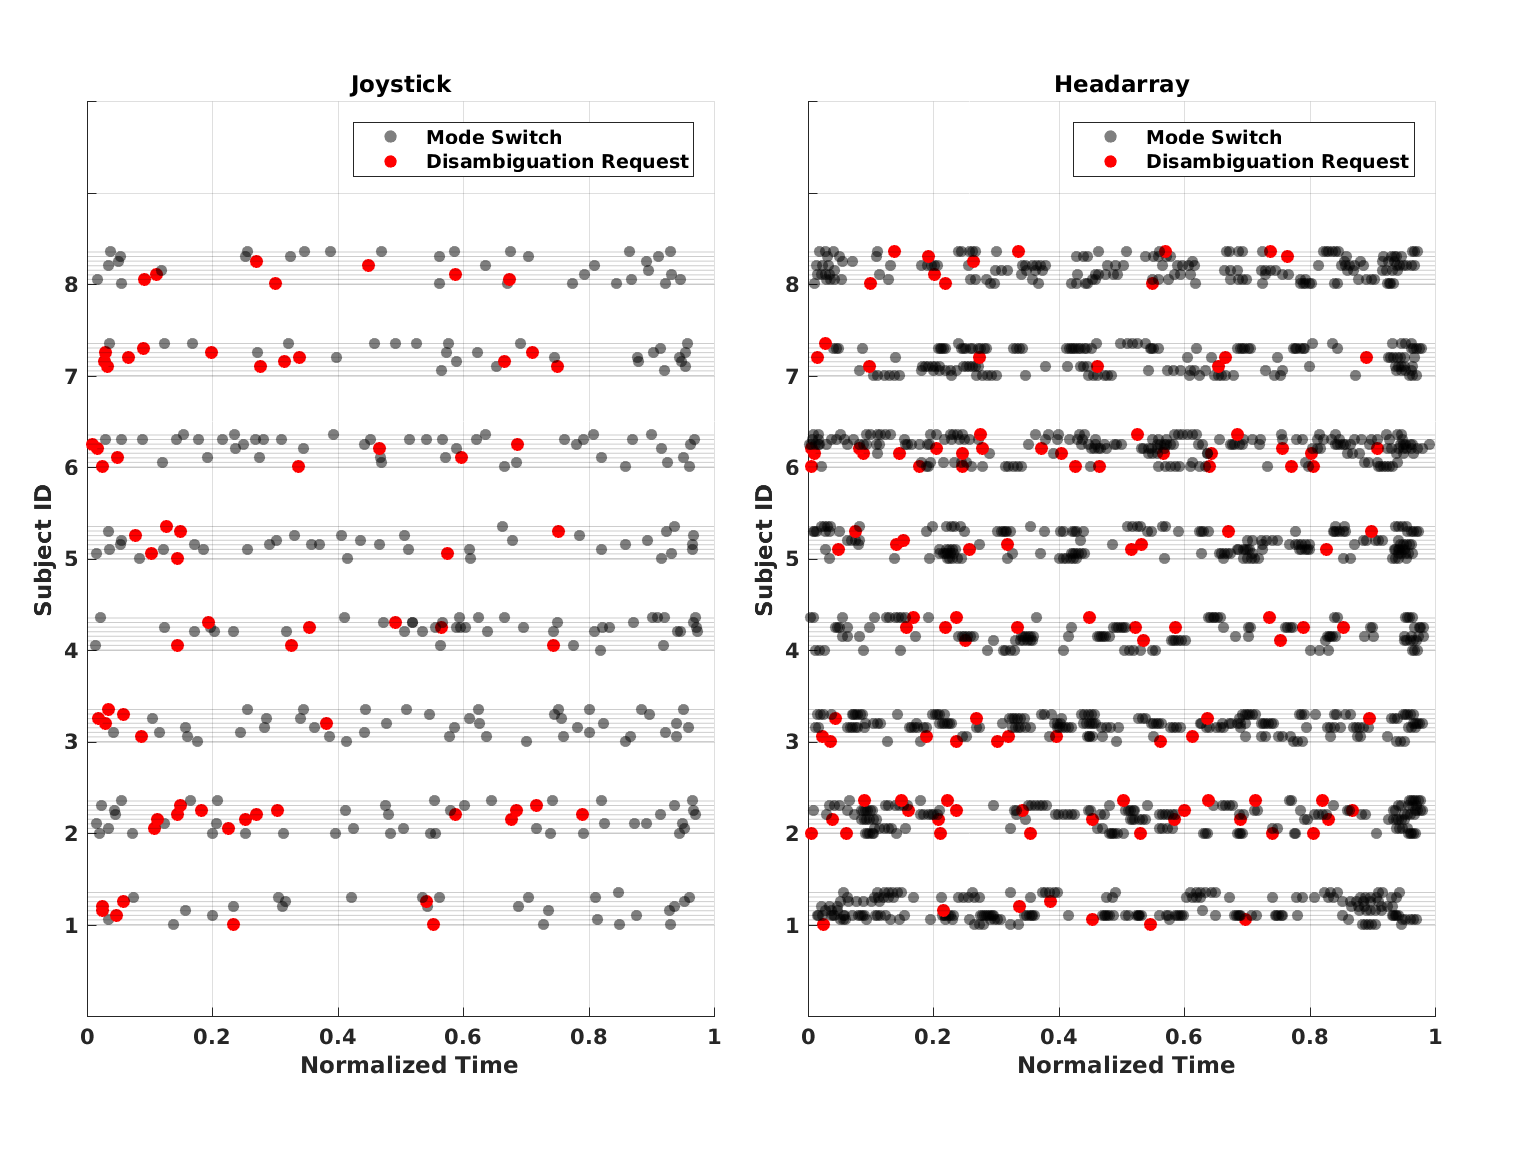
\includegraphics[width = 0.5\textwidth,center]{./figures/Fig9.eps}
	\vspace{-1cm}
	\caption{Temporal pattern of button presses for each interface and the multi-step task on a trial-by-trial basis for all subjects. Eight trials per subject per interface/task combination. For each subject, each light gray horizontal line represents a single trial (8 trials in total).}
	\label{fig:ha_man_disamb}
\end{figure}

\noindent{\textbf{Impact of Disambiguation on Task Performance:}} A statistically significant decrease in the number of button presses was observed between the \textit{Manual} and \textit{Disambiguation} paradigms when using the headarray (Figure~\ref{fig:button_press}, Left). Due to the low-dimensionality of the headarray and cyclical nature of mode switching, the number of button presses required for task completion is inherently high. That the disambiguation paradigm was helpful in reducing the number of button presses likely is due to higher robot assistance in the disambiguating control mode and therefore reduced the need for subsequent user-initiated mode switches.
For the joystick, statistically significant differences between the two paradigms were observed for the number of manual mode switches  ($p < 0.05$). However, this gain was offset by the button presses that were required for disambiguation requests. When grouping by task, the general trend (although not statistically significant) of a decrease in the number of button presses was more pronounced for the more complex multi-step task (Figure~\ref{fig:button_press}, Right). 

These results suggest that disambiguation is more useful as the control interface becomes more limited and the task becomes more complex. Intuitively, intent prediction becomes harder for the robot when the control interface is low-dimensional and does not reveal a great deal about the user's underlying intent. By having the users operate the robot in the disambiguating mode, the robot is able to elicit more intent-expressive control commands from the human which in turn helps in accurate goal inference and subsequently appropriate robot assistance. 

\noindent{\textbf{Temporal Distribution of Disambiguation Requests:}} 
The temporal distribution of disambiguation requests refers to \textit{when} the subject requested assistance during the course of a trial.
\begin{table}[t]
	\centering
	\caption{Characterization of the temporal distribution of disambiguation requests. }
%		The values in the table denote the deviation of the temporal distribution from a uniform distribution. Smaller values mean more concentrated and earlier disambiguation requests. } 
	%	\vspace{0.1cm}
	\label{table:skewness}
	\begin{tabular}{|c|c|c|c|}
		\hline
		& Single Step & Multi Step \\
		\hline
		Joystick & 0.63 & 0.57 \\
		\hline
		Headarray & 0.35 & 0.22 \\
		\hline
	\end{tabular}
\end{table}
We observed that a higher number of disambiguation requests correlates with the more limited interface and complex task.

From Figure~\ref{fig:ha_man_disamb} it is clear that the frequency and density of button presses (disambiguation requests plus mode switches) are much higher for the more limited control interface. The subjects also demonstrated a diverse range of disambiguation request behaviors, for example in regards to both when during the execution requests were made and with what frequency (e.g., Subject 8 versus Subject 2, Joystick). The variation between subjects is likely due to various factors such as the user's comfort in operating the robot and understanding of the disambiguating mode's ability to recruit more assistance from the autonomy. The skewness of the temporal distribution of disambiguation requests revealed a higher concentration of during the earlier parts of a trial (Table~\ref{table:skewness}) for both interfaces and tasks. However, under headarray control the temporal distribution was less skewed as the need for disambiguation request persists throughout the trial due the extremely low-bandwidth of the interface.\footnote{A uniform temporal distribution corresponds to a trial in which the disambiguation requests are uniformly spread out during the course of task execution. The skewness of a uniform distribution of 0.}


\noindent{\textbf{Task Completion Times:}} 
\added{No statistical difference was observed in task completion times between the \textit{Manual} and \textit{Disambiguation} paradigm. However, the variance in the task completion times was lower in \textit{Disambiguation} paradigm indicating that the task performance was more consistent when robot control was performed in the disambiguating control modes chosen by the autonomy. Furthermore, the overall task success was $94.53\%$ (242 out of 256 trials). 10 out of the 14 unsuccessful trials happened during the multi-step task.}
\begin{figure}[h!]
	\centering
	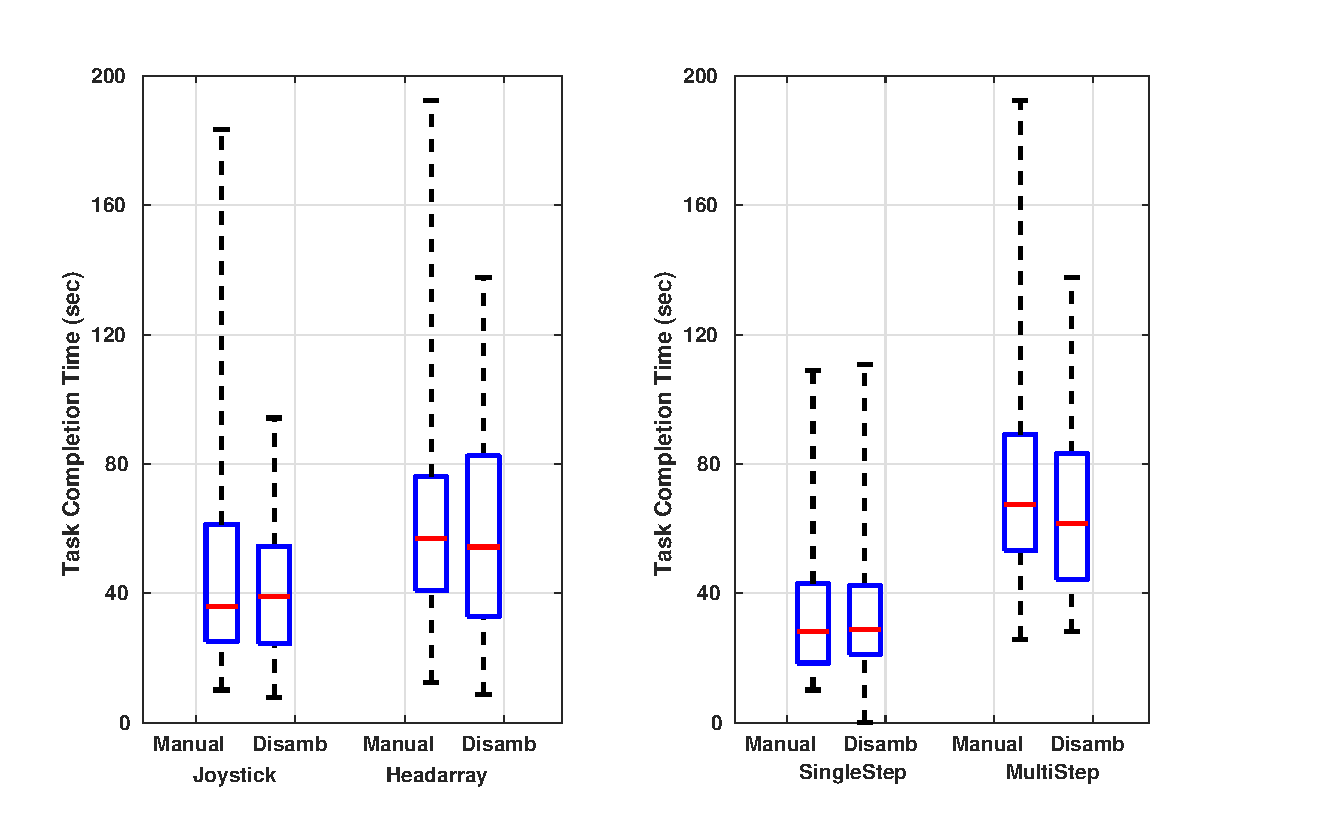
\includegraphics[width = 1\hsize, height=0.35\vsize, ,left]{./figures/task_completion.eps}
	\caption{Task completion times between \textit{Disambiguation} and \textit{Manual} Paradigms. \textit{Left:} Grouped by control interfaces. \textit{Right:} Grouped by tasks.}
	\label{fig:task_completion}
\end{figure}

\noindent{\textbf{User Survey Results:}} 
\added{Table~\ref{table:survey_results} summarizes the results of the subject survey. Users rated the utility value of the disambiguation paradigm (\textbf{Q1}) fairly high (4.87$\pm$0.95) indicating that task execution was easier during disambiguating trials. User responses strongly validated the effectiveness of the blending-based shared control scheme (\textbf{Q3}, 6.19$\pm$0.75). The responses also showed that subjects liked to operate the robot (\textbf{Q2}) in the disambiguating modes (5.00$\pm$1.15) and overwhelming preferred (\textbf{Q6}) the \textit{Disambiguation} to the \textit{Manual} paradigm. Unsurprisingly, all users felt that it was harder to control the robot using the headarray (\textbf{Q4}) and rated the utility value of the disambiguation paradigm to be higher for robot control with the headarray (\textbf{Q5}). Only four out of the eight subjects found the \textit{Disambiguation} paradigm to be user-friendly (\textbf{Q7}) likely due to the lack of transparency in why the autonomy chose the disambiguation mode.}

\begin{table}[t]
	\centering
	\caption{Subjective Survey Results}
	%		The values in the table denote the deviation of the temporal distribution from a uniform distribution. Smaller values mean more concentrated and earlier disambiguation requests. } 
	%	\vspace{0.1cm}
	\label{table:survey_results}
	\begin{tabular}{|c|c|c|c|}
		\hline
		& Across Tasks & Single-step & Multi-step \\
		\hline
		\textbf{Q1} & 4.87 $\pm$ 0.95  & 4.88 $\pm$ 0.99 & 4.88 $\pm$ 0.99 \\
		\hline
		\textbf{Q2} & 5.00 $\pm 1.15 $ & 5.25 $\pm$ 1.28 & 4.75 $\pm$ 1.03 \\
		\hline
		\textbf{Q3} & 6.19 $\pm$ 0.75 & 6.25 $\pm$ 0.89 & 6.13 $\pm$ 0.64 \\
		\hline
		\textbf{Q4} & Head Array  & Head Array  & Head Array  \\
		\hline
		\textbf{Q5} & Head Array  & Head Array  & Head Array  \\
		\hline
		\textbf{Q6} & Disambiguation & Disambiguation & Disambiguation \\
		\hline
		\textbf{Q7} & Disamb/Manual & Disamb/Manual & Disamb/Manual\\
		
		\hline
	\end{tabular}
\end{table}
%\noindent{\textbf{Onset of Robot Assistance:}} One of the motivations for developing the disambiguation system was that more accurate intent inference (as a result of intent disambiguation) should allow the autonomy to step in earlier more during the course of task execution. However, our results did not reveal any differences between the two switching paradigms across tasks or across interfaces
%\begin{figure}[h!]
%	\centering
%	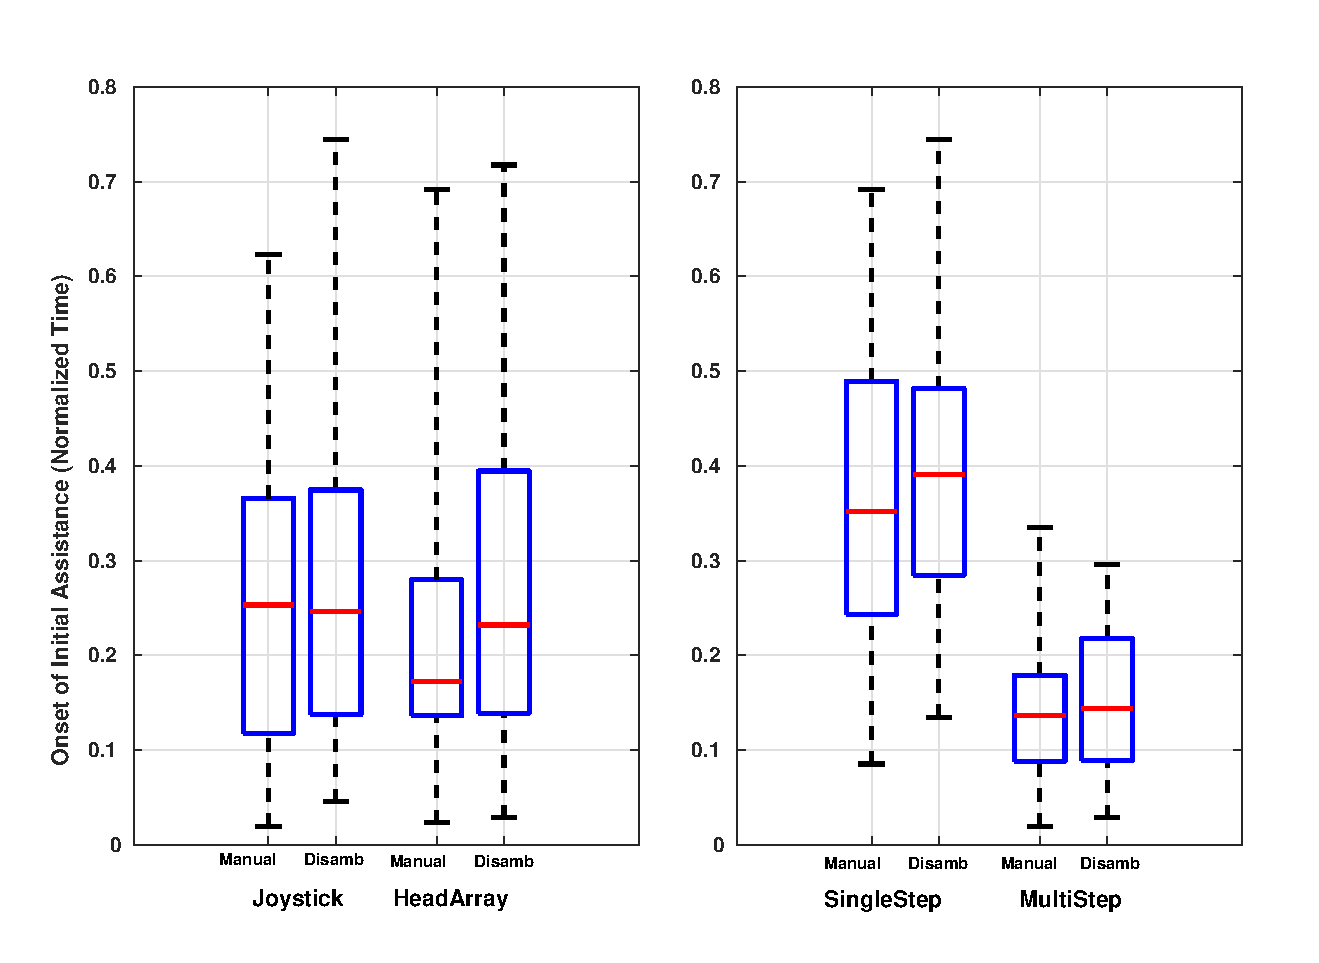
\includegraphics[width = 1\hsize ,center]{./figures/Fig10.eps}
%	\caption{Onset of robot assistance normalized with respect to task completion time. \textit{Left:} Across interfaces. \textit{Right:} Across tasks.}
%	\label{fig:initial_blend}
%\end{figure}
%One likely contributing factor is that disambiguation frequently was impaired by subjects choosing not to operate in the disambiguation mode after making a disambiguation request. One likely contributing factor is that disambiguation frequently was impaired by subjects choosing not to operate in the disambiguation mode after making a request. The disambiguation power of a control mode depends entirely on the observation of motion within that mode, and so in such scenarios disambiguation is effectively rendered inert.

\section{Discussion}\label{sec:discussion}
The disambiguation algorithm presented in our work can be utilized in any human-robot system in which there is a need to disambiguate between the different states a discrete hidden variable can assume (for example, a discrete set of goals in robotic manipulation or a set of landmarks in navigation tasks). Our algorithm assumes the existence of a discrete set of parameters (for example, control modes for robotic manipulation or natural language-based queries for navigation) that can help the intent inference mechanism to precisely converge to the correct inference. Although the disambiguation algorithm is task-agnostic---because it relies exclusively on the shape features of the probability distribution over the hidden variable---the disambiguation is only as good as the efficacy of the intent inference algorithm that is used for as specific task. In our experience, it becomes important that the choice of cost functions and domain-specific heuristics is appropriate for the task at hand. 

The efficacy of the disambiguation algorithm degraded when we used only a subset of the four features to inform the disambiguation metric. This only reinforces the need for a combination of different shape features for successful disambiguation.
\begin{figure}[h!]
	\centering
	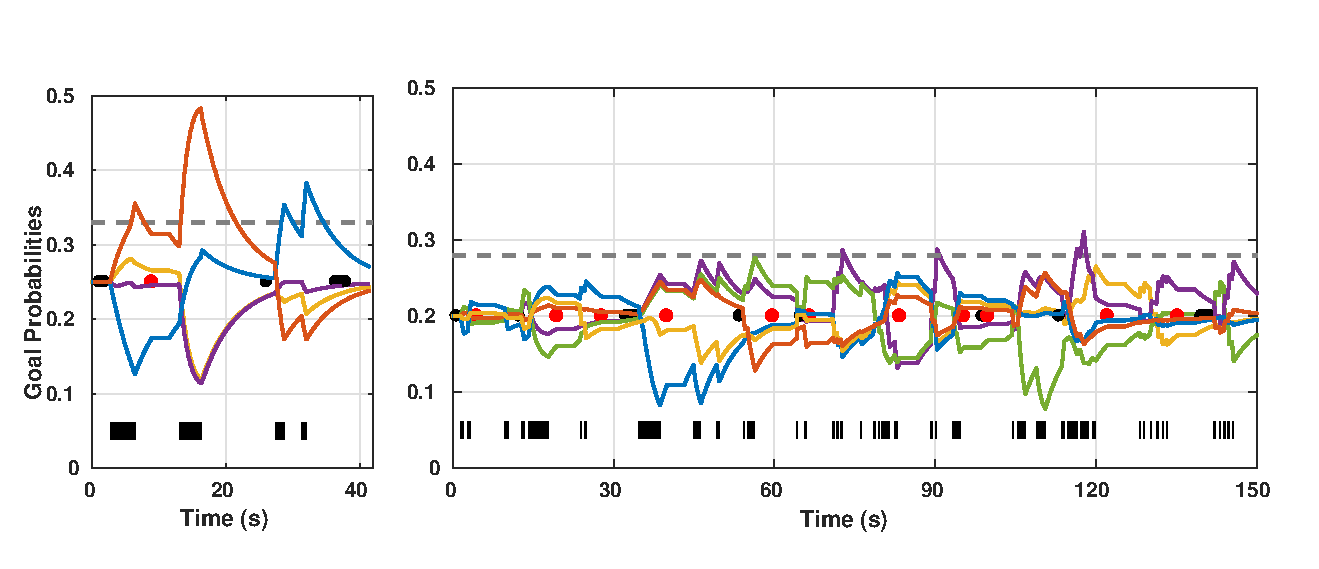
\includegraphics[width = 1\hsize, ,center]{./figures/Fig11.eps}
	\caption{Time evolution of goal probabilities. \textit{Top:} Multi-step task. \textit{Bottom:} Single-step task. The gray horizontal dashed line above denotes the minimum threshold for robot assistance. The black horizontal bars at the bottom denote non-zero human control commands. The red and black dots indicate button presses that are disambiguation requests and mode switches respectively. }
	\label{fig:gp_evolution}
\end{figure}
One observation from our subject study was how often participants submitted a disambiguation request and then chose not to operate in the selected mode---effectively not letting the robot help them. Our preliminary analysis showed that even though the autonomy was in a control mode that could have helped it perform accurate intent inference and subsequently assist the human, the user was not able to capitalize on it and utilize it to his/her advantage. As a result no differences in the onset of assistance was observed between the two switching paradigms across tasks or across interfaces.
This phenomenon is illustrated in Figure~\ref{fig:gp_evolution}. When control commands are issued, they are indicated by the black horizontal bars at the bottom of the plots. Disambiguation requests are shown as red dots, and mode switches as black dots. In plot on the right, we see multiple instances of disambiguation requests followed by no control commands or only very brief control commands. Another interesting behavior is shown in the left plot, where operation in the disambiguating mode very quickly elevates one goal probability above the threshold for providing autonomy assistance, and after the assistance kicks in the subject elects to stop issuing control commands.

This highlights the need for greater transparency in the human-robot interaction, so that the human has a clear picture of \textit{how} and \textit{why} the robot chooses to help the user in certain ways. A lack of understanding of how they might help the robot to help them might have resulted in the under-utilization of the disambiguation feature. In order to provide \textit{intent-expressive} control commands to the robot, very likely knowledge of the assistance mechanism is critical.  
%\added{Important to note is that this work was not about having the system select a control mode that the \textit{human} wants to use to reach a target (which might be motivated by a wide variety of factors such as line of sight or ease of use). In spite of this, subject responses to the user survey indicated that majority of the subjects liked operating the robot in the disambiguating modes and felt that task execution became easier as a result.} 
Therefore, the need for extensive and thorough training becomes apparent.
The training can be made more effective in a few different ways. First, online feedback of the robot's intent prediction at all times during training can likely help the subject gain a better understanding of the relationship between the characteristics of their control actions (sparsity, aggressiveness, persistence) and the robot's assistive behavior. Second, the subjects could be explicitly informed of the task relevant features (directedness, proximity \textit{et cetera}) that the robot relies on for determining the amount of assistance. Knowledge of these features might motivate the users to leverage the disambiguating mode. 

The inherent time delays associated with the computation of the disambiguating mode (approximately 2-2.5s) might have been a discouraging factor and a cause for user frustration \added{as a result of which half of the subjects thought the disambiguating system was not user-friendly}. The algorithm could be used to pre-compute a large set of most informative modes for different parts of the workspace, goal configurations and priors ahead of time, which then might be used a lookup table during task execution. 
Furthermore, metamodeling techniques and machine learning tools can be used to learn generalizable models that will be effective in previously unseen goal configurations. 

Automated mode switching schemes that eliminate the need for manual button presses altogether might also be a viable option for reducing task effort significantly.

%In the present system, there is task effort associated with requesting disambiguation assistance, which also might discourage the users from utilizing the paradigm. An improvement would be automated mode switching schemes that eliminate the need for button presses for disambiguation requests. 
%We also identify an opportunity to have adaptive assistance
%paradigms that explicitly take into account the characteristics of the user's control behavior. 
%Some users are timid in their operation of the robot whereas some others are more aggressive and confident. Some are more comfortable operating the robot manually and do not seek assistance, whereas some others rely on assistance more frequently. Individual user characteristics could be extracted from training and be used for tuning the parameters of the intent inference engine and the shared control system to maximize robustness and efficacy of the assistive system. This would also likely improve user satisfaction and result in higher user acceptance.

\section{Conclusion}\label{sec:conclusions}
In this paper, we have presented an algorithm for \textit{intent disambiguation assistance} with a shared-control robotic arm using the notion of \textit{inverse legibility}. The goal of our algorithm is to elicit more \textit{intent-expressive} control commands from the user by placing control in those control modes that \textit{maximally disambiguate} between the various goals in the scene. As a secondary contribution, we also present a novel intent inference mechanism inspired by \textit{dynamic field theory} that works in conjunction with the disambiguation system. A pilot user study was conducted with eight subjects to evaluate the efficacy of the disambiguation system. Our results indicate a decrease in task effort in terms of the number of button presses when disambiguation system employed. 

In our future work, as informed by our pilot study, we plan to extend the framework into an automated mode switch assistance system and  a more extensive user study with motor-impaired subjects will also be conducted.
%
%
%
%\appendices
%\section{Proof of the First Zonklar Equation}
%Appendix one text goes here.
%
%% you can choose not to have a title for an appendix
%% if you want by leaving the argument blank
%\section{}
%Appendix two text goes here.


% use section* for acknowledgment
\section*{Acknowledgment}
This material is based upon work supported by the National Science Foundation under Grant CNS 1544741. Any opinions, findings and conclusions or
recommendations expressed in this material are those of the authors and do
not necessarily reflect the views of the aforementioned institutions.



% Can use something like this to put references on a page
% by themselves when using endfloat and the captionsoff option.
%\ifCLASSOPTIONcaptionsoff
%  \newpage
%\fi



% trigger a \newpage just before the given reference
% number - used to balance the columns on the last page
% adjust value as needed - may need to be readjusted if
% the document is modified later
%\IEEEtriggeratref{8}
% The "triggered" command can be changed if desired:
%\IEEEtriggercmd{\enlargethispage{-5in}}

% references section

% can use a bibliography generated by BibTeX as a .bbl file
% BibTeX documentation can be easily obtained at:
% http://mirror.ctan.org/biblio/bibtex/contrib/doc/
% The IEEEtran BibTeX style support page is at:
% http://www.michaelshell.org/tex/ieeetran/bibtex/
\balance
\bibliographystyle{IEEEtran}
% argument is your BibTeX string definitions and bibliography database(s)
\bibliography{references}

%
% <OR> manually copy in the resultant .bbl file
% set second argument of \begin to the number of references
% (used to reserve space for the reference number labels box)
%\begin{thebibliography}{1}
%
%\providecommand{\natexlab}[1]{#1}
%\providecommand{\url}[1]{{#1}}
%\providecommand{\urlprefix}{URL}
%\expandafter\ifx\csname urlstyle\endcsname\relax
%\providecommand{\doi}[1]{DOI~\discretionary{}{}{}#1}\else
%\providecommand{\doi}{DOI~\discretionary{}{}{}\begingroup
%	\urlstyle{rm}\Url}\fi
%\providecommand{\eprint}[2][]{\url{#2}}
%
%	
%
%
%%%%%%%%%%%%%%%%%%%%%%%%%%%%%%%%%%%%%%%%%55
%	\providecommand{\natexlab}[1]{#1}
%\providecommand{\url}[1]{{#1}}
%\providecommand{\urlprefix}{URL}
%\expandafter\ifx\csname urlstyle\endcsname\relax
%\providecommand{\doi}[1]{DOI~\discretionary{}{}{}#1}\else
%\providecommand{\doi}{DOI~\discretionary{}{}{}\begingroup
%	\urlstyle{rm}\Url}\fi
%\providecommand{\eprint}[2][]{\url{#2}}
%
%\bibitem{admoni2016predicting}
%Admoni H, Srinivasa S (2016) Predicting user intent through eye gaze for shared
%autonomy. In: Proceedings of the AAAI Fall Symposium Series: Shared Autonomy
%in Research and Practice (AAAI Fall Symposium), pp 298--303
%
%\bibitem{amari1977dynamics}
%Amari Si (1977) Dynamics of pattern formation in lateral-inhibition type neural
%fields. \textit{Biological Cybernetics} 27(2):77--87
%
%\bibitem{argall2009survey}
%Argall BD, Chernova S, Veloso M, Browning B (2009) A survey of robot learning
%from demonstration. \textit{Robotics and Autonomous Systems} 57(5):469--483
%
%\bibitem{atanasov2014information}
%Atanasov N, Le~Ny J, Daniilidis K, Pappas GJ (2014) Information acquisition
%with sensing robots: Algorithms and error bounds. In: \textit{Proceedings of
%	the IEEE International Conference on Robotics and Automation (ICRA)}
%
%\bibitem{barrett2005accurate}
%Barrett CH, Todd PM, Miller GF, Blythe PW (2005) Accurate judgments of
%intention from motion cues alone: A cross-cultural study. \textit{Evolution
%	and Human Behavior} 26(4):313--331
%
%\bibitem{choi2008laser}
%Choi YS, Anderson CD, Glass JD, Kemp CC (2008) Laser pointers and a touch
%screen: intuitive interfaces for autonomous mobile manipulation for the motor
%impaired. In: \textit{Proceedings of the International SIGACCESS Conference
%	on Computers and Accessibility}
%
%\bibitem{demeester2008user}
%Demeester E, H{\"u}ntemann A, Vanhooydonck D, Vanacker G, Van~Brussel H, Nuttin
%M (2008) User-adapted plan recognition and user-adapted shared control: A
%bayesian approach to semi-autonomous wheelchair driving. \textit{Autonomous
%	Robots} 24(2):193--211
%
%\bibitem{downey2016blending}
%Downey JE, Weiss JM, Muelling K, Venkatraman A, Valois JS, Hebert M, Bagnell
%JA, Schwartz AB, Collinger JL (2016) Blending of brain-machine interface and
%vision-guided autonomous robotics improves neuroprosthetic arm performance
%during grasping. \textit{Journal of Neuroengineering and Rehabilitation}
%13(1):28
%
%\bibitem{dragan2012assistive}
%Dragan AD, Srinivasa SS (2012{\natexlab{a}}) Assistive teleoperation for
%manipulation tasks. In: \textit{Proceedings of ACM/IEEE International
%	Conference on Human-Robot Interaction (HRI)}
%
%\bibitem{dragan2012formalizing}
%Dragan AD, Srinivasa SS (2012{\natexlab{b}}) Formalizing assistive
%teleoperation. MIT Press
%
%\bibitem{dragan2013policy}
%Dragan AD, Srinivasa SS (2013) A policy-blending formalism for shared control.
%\textit{The International Journal of Robotics Research} 32(7):790--805
%
%\bibitem{dragan2013legibility}
%Dragan AD, Lee KC, Srinivasa SS (2013) Legibility and predictability of robot
%motion. In: \textit{Proceedings of the ACM/IEEE International Conference on
%	Human-Robot Interaction (HRI)}
%
%\bibitem{driessen2005collaborative}
%Driessen B, Kate TT, Liefhebber F, Versluis A, Van~Woerden J (2005)
%Collaborative control of the manus manipulator. \textit{Universal Access in
%	the Information Society} 4(2):165--173
%
%\bibitem{eftring1999technical}
%Eftring H, Boschian K (1999) Technical results from manus user trials. In:
%\textit{IEEE 2nd International Conference on Rehabilitation Robotics (ICORR)}
%
%\bibitem{erlhagen2006dynamic}
%Erlhagen W, Bicho E (2006) The dynamic neural field approach to cognitive
%robotics. \textit{Journal of Neural Engineering} 3(3):R36
%
%\bibitem{erlhagen2014dynamic}
%Erlhagen W, Bicho E (2014) A dynamic neural field approach to natural and
%efficient human-robot collaboration. In: \textit{Neural Fields}, Springer, pp
%341--365
%
%\bibitem{faubel2008learning}
%Faubel C, Sch{\"o}ner G (2008) Learning to recognize objects on the fly: a
%neurally based dynamic field approach. \textit{Neural Networks}
%21(4):562--576
%
%\bibitem{goodfellow2010help}
%Goodfellow IJ, Koenig N, Muja M, Pantofaru C, Sorokin A, Takayama L (2010) Help
%me help you: Interfaces for personal robots. In: \textit{Proceedings of
%	ACM/IEEE International Conference on Human-Robot Interaction (HRI)}
%
%\bibitem{gopinath2017mode}
%Gopinath D, Argall B (2017) Mode switch assistance to maximize human intent
%disambiguation. In: \textit{Robotics: Science and Systems}
%
%\bibitem{gopinath2017human}
%Gopinath D, Jain S, Argall BD (2017) Human-in-the-loop optimization of shared
%autonomy in assistive robotics. \textit{IEEE Robotics and Automation Letters}
%2(1):247--254
%
%\bibitem{herlant2016assistive}
%Herlant LV, Holladay RM, Srinivasa SS (2016) Assistive teleoperation of robot
%arms via automatic time-optimal mode switching. In: \textit{Proceedings of
%	the ACM/IEEE International Conference on Human-Robot Interaction (HRI)}
%
%\bibitem{holladay2014legible}
%Holladay RM, Dragan AD, Srinivasa SS (2014) Legible robot pointing. In:
%\textit{The IEEE International Symposium on Robot and Human Interactive
%	Communication (RO-MAN)}
%
%\bibitem{hsu2002randomized}
%Hsu D, Kindel R, Latombe JC, Rock S (2002) Randomized kinodynamic motion
%planning with moving obstacles. \textit{The International Journal of Robotics
%	Research} 21(3):233--255
%
%\bibitem{huete2012personal}
%Huete AJ, Victores JG, Martinez S, Gim{\'e}nez A, Balaguer C (2012) Personal
%autonomy rehabilitation in home environments by a portable assistive robot.
%\textit{IEEE Transactions on Systems, Man, and Cybernetics, Part C
%	(Applications and Reviews)} 42(4):561--570
%
%\bibitem{javdani2017shared}
%Javdani S, Admoni H, Pellegrinelli S, Srinivasa SS, Bagnell JA (2017) Shared
%autonomy via hindsight optimization for teleoperation and teaming. arXiv
%preprint arXiv:170600155
%
%\bibitem{kelley2008understanding}
%Kelley R, Tavakkoli A, King C, Nicolescu M, Nicolescu M, Bebis G (2008)
%Understanding human intentions via hidden markov models in autonomous mobile
%robots. In: \textit{Proceedings of the 3rd ACM/IEEE International Conference
%	on Human Robot Interaction}, ACM, pp 367--374
%
%\bibitem{khatib1986real}
%Khatib O (1986) Real-time obstacle avoidance for manipulators and mobile
%robots. \textit{The International Journal of Robotics Research} 5(1):90--98
%
%\bibitem{kim2010relationship}
%Kim DJ, Hazlett R, Godfrey H, Rucks G, Portee D, Bricout J, Cunningham T, Behal
%A (2010) On the relationship between autonomy, performance, and satisfaction:
%Lessons from a three-week user study with post-sci patients using a smart
%6dof assistive robotic manipulator. In: \textit{Proceeding of the IEEE
%	International Conference on Robotics and Automation (ICRA)}, IEEE, pp
%217--222
%
%\bibitem{kim2012autonomy}
%Kim DJ, Hazlett-Knudsen R, Culver-Godfrey H, Rucks G, Cunningham T, Portee D,
%Bricout J, Wang Z, Behal A (2012) How autonomy impacts performance and
%satisfaction: Results from a study with spinal cord injured subjects using an
%assistive robot. \textit{IEEE Transactions on Systems, Man, and
%	Cybernetics-Part A: Systems and Humans} 42(1):2--14
%
%\bibitem{laplante1992assistive}
%LaPlante MP, et~al (1992) Assistive technology devices and home accessibility
%features: prevalence, payment, need, and trends. \textit{Advance Data from
%	Vital and Health Statistics}
%
%\bibitem{liu2016goal}
%Liu C, Hamrick JB, Fisac JF, Dragan AD, Hedrick JK, Sastry SS, Griffiths TL
%(2016) Goal inference improves objective and perceived performance in
%human-robot collaboration. In: \textit{Proceedings of the 2016 International
%	Conference on Autonomous Agents \& Multiagent Systems}, International
%Foundation for Autonomous Agents and Multiagent Systems, pp 940--948
%
%\bibitem{miller2013trajectory}
%Miller LM, Murphey TD (2013) Trajectory optimization for continuous ergodic
%exploration. In: \textit{American Control Conference (ACC)}
%
%\bibitem{miller2016ergodic}
%Miller LM, Silverman Y, MacIver MA, Murphey TD (2016) Ergodic exploration of
%distributed information. \textit{IEEE Transactions on Robotics} 32(1):36--52
%
%\bibitem{muelling2017autonomy}
%Muelling K, Venkatraman A, Valois JS, Downey JE, Weiss J, Javdani S, Hebert M,
%Schwartz AB, Collinger JL, Bagnell JA (2017) Autonomy infused teleoperation
%with application to brain computer interface controlled manipulation.
%\textit{Autonomous Robots} pp 1--22
%
%\bibitem{nuttin2002selection}
%Nuttin M, Vanhooydonck D, Demeester E, Van~Brussel H (2002) Selection of
%suitable human-robot interaction techniques for intelligent wheelchairs. In:
%\textit{Proceedings of 11th IEEE International Workshop on Robot and Human
%	Interactive Communication}, IEEE, pp 146--151
%
%\bibitem{pellegrinelli2016human}
%Pellegrinelli S, Admoni H, Javdani S, Srinivasa S (2016) Human-robot shared
%workspace collaboration via hindsight optimization. In: 2016 IEEE/RSJ International Conference on Intelligent Robots
%and Systems (IROS), IEEE, pp
%831--838
%
%\bibitem{philips2007adaptive}
%Philips J, Mill{\'a}n JdR, Vanacker G, Lew E, Gal{\'a}n F, Ferrez PW,
%Van~Brussel H, Nuttin M (2007) Adaptive shared control of a brain-actuated
%simulated wheelchair. In: \textit{Proceedings of the IEEE International
%	Conference on Rehabilitation Robotics (ICORR)}, IEEE, pp 408--414
%
%\bibitem{pilarski2012dynamic}
%Pilarski PM, Dawson MR, Degris T, Carey JP, Sutton RS (2012) Dynamic switching
%and real-time machine learning for improved human control of assistive
%biomedical robots. In: \textit{Proceedings of the IEEE RAS \& EMBS
%	International Conference on Biomedical Robotics and Biomechatronics (BioRob)
%}, IEEE, pp 296--302
%
%\bibitem{ratliff2009chomp}
%Ratliff N, Zucker M, Bagnell JA, Srinivasa S (2009) Chomp: Gradient
%optimization techniques for efficient motion planning. In:
%\textit{Proceedings of the IEEE International Conference on Robotics and
%	Automation (ICRA)}, IEEE, pp 489--494
%
%\bibitem{rimon1992exact}
%Rimon E, Koditschek DE (1992) Exact robot navigation using artificial potential
%functions. \textit{IEEE Transactions on Robotics and Automation}
%8(5):501--518
%
%\bibitem{sadigh2016information}
%Sadigh D, Sastry SS, Seshia SA, Dragan A (2016) Information gathering actions
%over human internal state. In: \textit{Proceedings of the IEEE/RSJ
%	International Conference on Intelligent Robots and Systems (IROS)}, IEEE, pp
%66--73
%
%\bibitem{schaal1997learning}
%Schaal S (1997) Learning from demonstration. In: \textit{Advances in Neural
%	Information Processing Systems}, pp 1040--1046
%
%\bibitem{scherer1996outcomes}
%Scherer MJ (1996) Outcomes of assistive technology use on quality of life.
%\textit{Disability and Rehabilitation} 18(9):439--448
%
%\bibitem{schoner2008dynamical}
%Sch{\"o}ner G (2008) Dynamical systems approaches to cognition.
%\textit{Cambridge Handbook of Computational Cognitive Modeling} pp 101--126
%
%\bibitem{schoner2015dynamic}
%Sch{\"o}ner G, Spencer J (2015) \textit{Dynamic thinking: A primer on dynamic
%	field theory}. Oxford University Press
%
%\bibitem{schoner1995dynamics}
%Sch{\"o}ner G, Dose M, Engels C (1995) Dynamics of behavior: Theory and
%applications for autonomous robot architectures. \textit{Robotics and
%	Autonomous Systems} 16(2-4):213--245
%
%\bibitem{simpson2008tooth}
%Simpson T, Broughton C, Gauthier MJ, Prochazka A (2008) Tooth-click control of
%a hands-free computer interface. \textit{IEEE Transactions on Biomedical
%	Engineering} 55(8):2050--2056
%
%\bibitem{sorokin2010people}
%Sorokin A, Berenson D, Srinivasa SS, Hebert M (2010) People helping robots
%helping people: Crowdsourcing for grasping novel objects. In:
%\textit{Proceedings of the IEEE/RSJ International Conference on Intelligent
%	Robots and Systems (IROS)}
%
%\bibitem{storms2014blending}
%Storms JG, Tilbury DM (2014) Blending of human and obstacle avoidance control
%for a high speed mobile robot. In: \textit{American Control Conference
%	(ACC)}, IEEE, pp 3488--3493
%
%\bibitem{tanner2003nonholonomic}
%Tanner HG, Loizou SG, Kyriakopoulos KJ (2003) Nonholonomic navigation and
%control of cooperating mobile manipulators. \textit{IEEE Transactions on
%	Robotics and Automation} 19(1):53--64
%
%\bibitem{tsui2011want}
%Tsui KM, Kim DJ, Behal A, Kontak D, Yanco HA (2011) “{I} want that”:
%Human-in-the-loop control of a wheelchair-mounted robotic arm.
%\textit{Applied Bionics and Biomechanics} 8(1):127--147
%
%\bibitem{wang2013probabilistic}
%Wang Z, M{\"u}lling K, Deisenroth MP, Ben~Amor H, Vogt D, Sch{\"o}lkopf B,
%Peters J (2013) Probabilistic movement modeling for intention inference in
%human--robot interaction. \textit{The International Journal of Robotics
%	Research} 32(7):841--858
%
%\bibitem{zibner2011dynamic}
%Zibner SK, Faubel C, Iossifidis I, Schoner G (2011) Dynamic neural fields as
%building blocks of a cortex-inspired architecture for robotic scene
%representation. \textit{IEEE Transactions on Autonomous Mental Development}
%3(1):74--91
%
%\bibitem{ziebart2008maximum}
%Ziebart BD, Maas AL, Bagnell JA, Dey AK (2008) Maximum entropy inverse
%reinforcement learning. In: AAAI, Chicago, IL, USA, vol~8, pp 1433--1438
%\end{thebibliography}

% biography section
% 
% If you have an EPS/PDF photo (graphicx package needed) extra braces are
% needed around the contents of the optional argument to biography to prevent
% the LaTeX parser from getting confused when it sees the complicated
% \includegraphics command within an optional argument. (You could create
% your own custom macro containing the \includegraphics command to make things
% simpler here.)
%\begin{IEEEbiography}[{\includegraphics[width=1in,height=1.25in,clip,keepaspectratio]{mshell}}]{Michael Shell}
% or if you just want to reserve a space for a photo:

%\begin{IEEEbiography}{Michael Shell}
%Biography text here.
%\end{IEEEbiography}
%
%% if you will not have a photo at all:
%\begin{IEEEbiographynophoto}{John Doe}
%Biography text here.
%\end{IEEEbiographynophoto}
%
%% insert where needed to balance the two columns on the last page with
%% biographies
%%\newpage
%
%\begin{IEEEbiographynophoto}{Jane Doe}
%Biography text here.
%\end{IEEEbiographynophoto}

% You can push biographies down or up by placing
% a \vfill before or after them. The appropriate
% use of \vfill depends on what kind of text is
% on the last page and whether or not the columns
% are being equalized.

%\vfill

% Can be used to pull up biographies so that the bottom of the last one
% is flush with the other column.
%\enlargethispage{-5in}



% that's all folks
\end{document}


